\documentclass[10pt,a4paper]{article}
\usepackage[UTF8,fontset = windows]{ctex}
\setCJKmainfont[BoldFont=黑体,ItalicFont=楷体]{华文中宋}
\usepackage{amssymb,amsmath,amsfonts,amsthm,mathrsfs,dsfont,graphicx}
\usepackage{ifthen,indentfirst,enumerate,color,titletoc}
\usepackage{tikz}
\usepackage{makecell}
\usepackage{longtable}
%\usepackage{mathptmx}

\usetikzlibrary{arrows,calc,intersections,patterns,decorations.pathreplacing,angles,quotes}
\usepackage[bf,small,indentafter,pagestyles]{titlesec}
\usepackage[top=1in, bottom=1in,left=0.8in,right=0.8in]{geometry}
\renewcommand{\baselinestretch}{1.65}
\newtheorem{defi}{定义~}
\newtheorem{eg}{例~}
\newtheorem{ex}{~}
\newtheorem{rem}{注~}
\newtheorem{thm}{定理~}
\newtheorem{coro}{推论~}
\newtheorem{axiom}{公理~}
\newtheorem{prop}{性质~}
\newcommand{\blank}[1]{\underline{\hbox to #1pt{}}}
\newcommand{\bracket}[1]{(\hbox to #1pt{})}
\newcommand{\onech}[4]{\par\begin{tabular}{p{.9\textwidth}}
A.~#1\\
B.~#2\\
C.~#3\\
D.~#4
\end{tabular}}
\newcommand{\twoch}[4]{\par\begin{tabular}{p{.46\textwidth}p{.46\textwidth}}
A.~#1& B.~#2\\
C.~#3& D.~#4
\end{tabular}}
\newcommand{\vartwoch}[4]{\par\begin{tabular}{p{.46\textwidth}p{.46\textwidth}}
(1)~#1& (2)~#2\\
(3)~#3& (4)~#4
\end{tabular}}
\newcommand{\fourch}[4]{\par\begin{tabular}{p{.23\textwidth}p{.23\textwidth}p{.23\textwidth}p{.23\textwidth}}
A.~#1 &B.~#2& C.~#3& D.~#4
\end{tabular}}
\newcommand{\varfourch}[4]{\par\begin{tabular}{p{.23\textwidth}p{.23\textwidth}p{.23\textwidth}p{.23\textwidth}}
(1)~#1 &(2)~#2& (3)~#3& (4)~#4
\end{tabular}}
\begin{document}
\begin{enumerate}[1.]


\item 已知数列$\{a_n\}$的通项公式为$a_n=2(1+3n)$, 填写下表:
\begin{center}
    \begin{tabular}{|p{.05\textwidth}<{\centering}|p{.05\textwidth}<{\centering}|p{.05\textwidth}<{\centering}|p{.05\textwidth}<{\centering}|p{.05\textwidth}<{\centering}|p{.05\textwidth}<{\centering}|p{.05\textwidth}<{\centering}|p{.05\textwidth}<{\centering}|p{.05\textwidth}<{\centering}|p{.05\textwidth}<{\centering}|}
        \hline
        $n$ & $1$ & $2$ & $3$ & $\cdots$ & $11$ & $\cdots$ & & $\cdots$ & \\ \hline
        $a_n$ & & & & $\cdots$ & & $\cdots$ & $128$ & $\cdots$ & $602$ \\ \hline        
    \end{tabular}
\end{center}
在数列$-1,0,\dfrac 19,\dfrac 18,\cdots ,\dfrac{n-2}{n^2},\cdots$中, $\dfrac 2{25}$是它的第\blank{50}项.
\item 已知无穷数列$1\times 2,2\times 3,3\times 4,\cdots ,n(n+1),\cdots$.\\
(1) 求这个数列的第$10$项、第$31$项及第$48$项;\\
(2) $420$是不是这个数列的项? 如果是, 那么是第几项?
\item 写出下列数列的一个通项公式, 使它的前$4$项分别是下列各数:\\
(1) $4, 8, 12, 16$;\\
(2) $\dfrac 12,\dfrac 23,\dfrac 34,\dfrac 45$;\\
(3) $-\dfrac 1{2\times 1},\dfrac 1{2\times 2},-\dfrac 1{2\times 3},\dfrac 1{2\times 4}$;\\
(4) $1,-\sqrt[3]2,\sqrt[3]3,-\sqrt[3]4$.
\item 根据下面的图形及相应的点数在横线上画出适当的图形.
\begin{center}
    \begin{tikzpicture}[scale = 0.5]
        \filldraw (0,0) circle (0.05);
        \filldraw (2,0) circle (0.05) (3,0) circle (0.05) (2,0) ++ (60:1) circle (0.05);
        \filldraw (5,0) circle (0.05) (6,0) circle (0.05) (7,0) circle (0.05) (5,0) ++ (60:1) circle (0.05) ++ (1,0) circle (0.05) ++ (120:1) circle (0.05);
        \filldraw (9,0) circle (0.05) (10,0) circle (0.05) (11,0) circle (0.05) (12,0) circle (0.05) (9,0) ++ (60:1) circle (0.05) ++ (1,0) circle (0.05) ++ (1,0) circle (0.05) (9,0) ++ (60:2) circle (0.05) ++ (1,0) circle (0.05) ++ (120:1) circle (0.05);
    \end{tikzpicture}
    \blank{100}.
\end{center}
\item 根据下列条件, 分别写出数列$\{a_n\}$的前$5$项.\\
(1) $a_1=5$, $a_n=a_{n-1}+4$($n\ge 2$);\\
(2) $a_1=2$, $a_n=3a_{n-1}$($n\ge 2$);\\
(3) $a_1=1$, $a_n=a_{n-1}+\dfrac 1{a_{n-1}}$($n\ge 2$).
\item 根据下列条件, 分别写出数列$\{a_n\}$的第$3$项至第$5$项.\\
(1) $a_1=1$, $a_n=2a_{n-1}+3$;\\
(2) $a_1=1$, $a_n=2a_{n-1}+2^n$.
\item 写出数列: $\dfrac 12,\dfrac 38,\dfrac 5{18},\dfrac 7{32},\cdots$的一个通项公式.
\item 已知数列$\{a_n\}$满足: $a_1=1$, $a_{n+1}=a_n+n+1$.求$a_6$.
\item 已知数列$\{a_n\}$满足$a_n=\dfrac{n^2+n+1}3$.\\
(1) 写出$a_{10}$与$a_{n+1}$;\\
(2) $79\dfrac 23$是不是数列$\{a_n\}$的项? 如果是, 那么是第几项?
\item 已知数列$\{a_n\}$满足: $a_1=1$, $a_2=6$, $a_{n+2}=-a_n$.\\
(1) 写出这个数列的前$8$项;\\
(2) 根据第(1)题的结论, 猜想这个数列的项所具有的特征.
\item 判断下列数列中, 哪些是等差数列.是等差数列的, 请写出等差数列的公差$d$.\\
(1) $1, 11, 121$;\\
(2) $1, 2, 1$;\\
(3) $\lg 2,\lg 4,\lg 8$;\\
(4) $2, 2, 2$.
\item 已知数列$\{a_n\}$是等差数列, 请在下表中填入适当的数:
\begin{center}
    \begin{tabular}{|p{.15\textwidth}<{\centering}|p{.15\textwidth}<{\centering}|p{.15\textwidth}<{\centering}|p{.15\textwidth}<{\centering}|p{.15\textwidth}<{\centering}|}
        \hline
        $a_1$ & $a_2$ & $a_3$ & 公差$d$ & $a_5$ \\ \hline
        $-3$ & & $6$ & & \\ \hline
        & $-5$ & & $2$ & \\ \hline
    \end{tabular}
\end{center}
\item 根据所给的条件填写下表:
\begin{center}
    \begin{tabular}{|p{.15\textwidth}<{\centering}|p{.15\textwidth}<{\centering}|p{.15\textwidth}<{\centering}|p{.15\textwidth}<{\centering}|p{.15\textwidth}<{\centering}|}
        \hline
         & $a_1$ & $d$ & $n$ & $a_n$ \\ \hline
        等差数列$\{a_n\}$ & $5$ & $10$ & $12$ &  \\ \hline
        等差数列$\{a_n\}$ & $-5$ & $6$ & & $61$ \\ \hline
    \end{tabular}
\end{center}
\item 已知数列$\{a_n\}$是等差数列, 且$a_1+a_6=12$, $a_4=7$, 求这个数列的通项公式.
\item 已知数列$\{a_n\}$是等差数列, 且$a_7=2$, $a_8=-4$, 求$a_1$与$a_{10}$.
\item 已知数列$\{a_n\}$是等差数列, 且$a_6=4$, $a_{14}=64$.设$a_6$与$a_{14}$的等差中项为$x$, $a_6$与$x$的等差中项为$y$, $x$与$a_{14}$的等差中项为$z$, 求$x+y+z$.
\item 分别求下面两题中两数的等差中项:\\
(1) $\dfrac{8-\sqrt 2}2$与$\dfrac{8+\sqrt 2}2$;\\
(2) $(a+b)^2$与$(a-b)^2$.
\item 已知数列$\{a_n\}$是等差数列, 且$b_n=a_n+a_{n+1}$.求证: 数列$\{b_n\}$是等差数列.
\item 已知三个数成等差数列, 首末两项之积为中间项的$5$倍, 后两项的和为第一项的$8$倍, 求这三个数.
\item 已知非零实数$a,b,c$不全相等.如果$a,b,c$成等差数列, 那么$\dfrac 1a,\dfrac 1b,\dfrac 1c$能不能构成等差数列? 为什么?
\item 已知数列$\{a_n\}$是等差数列.\\
(1) $2a_5=a_4+a_6$是否成立? 为什么?\\
(2) 求证: $2a_n=a_{n-1}+a_{n+1}$($n\ge 2$);\\
(3) 由第(2)题你可以推广出怎样的结论?
\item 夏季高山上的温度从山脚起每升高$100$米降低$0.7^\circ\text{C}$.已知山脚的温度是$34.9^\circ\text{C}$, 山顶的温度是$23^\circ\text{C}$, 求山的相对高度.
\item 某产品按质量分成$10$个档次, 生产最低档次的利润是$8$元/件.每提高一个档次, 利润每件增加$2$元, 产量减少$3$件.如果在某段时间内, 最低档的产品可生产$60$件, 那么在相同时间内, 生产第几档次的产品可获得最大利润? (最低档次为第$1$档)
\item 已知等差数列$\{a_n\}$分别满足下列条件, 求解相应问题.\\
(1) $d=\dfrac 13$, $n=37$, $S_n=629$, 求$a_1$;\\
(2) $d=2$, $n=15$, $a_n=-10$, 求$S_n$;\\
(3) $a_1=20$, $a_n=54$, $S_n=999$, 求$d$;\\
(4) $a_1=\dfrac 56$, $d=-\dfrac 16$, $S_n=-5$, 求$a_n$.
\item 已知等差数列$\{a_n\}$的第$6$项是$5$, 第$3$项与第$8$项的和也是$5$, 求这个数列的前$9$项和.
\item 求$100$以内能被$7$整除的所有正整数的和.
\item 某礼堂有$18$排座位, 第$1$排有$26$个座位, 以后每一排都比前一排多$2$个座位.这个礼堂共能坐多少人?
\item 某单位开发了一个受政府扶持的新项目, 得到政府无息贷款$50$万元用于购买设备.已知该设备在使用过程中第一天使用费是$101$元, $\cdots$, 第$n$天的使用费是$(100+n)$元.如果总费用$=$购置费$+$使用费, 那么使用多少天后, 平均每天的费用最低?
\item 已知$a,b,c,d$成等差数列, 求证: $2a-3b$, $2b-3c$, $2c-3d$成等差数列.
\item 如果数列$\{a_n\}$、$\{b_n\}$是项数相同的两个等差数列, $p,q$是常数, 那么数列$\{pa_n+qb_n\}$是等差数列吗? 为什么?
\item 已知数列$\{a_n\}$的各项均不为零, 且$a_n=\dfrac{3a_{n-1}}{a_{n-1}+3}$($n\ge 2$), $b_n=\dfrac 1{a_n}$.求证: 数列$\{b_n\}$是等差数列.
\item 已知等差数列$\{a_n\}$的前$15$项和为$135$, 求这个数列的第$8$项.
\item 已知等差数列$\{a_n\}$的前$5$项和为$0$, 前$10$项和为$-100$, 求这个数列的前$20$项和.
\item 已知数列$\{a_n\}$的前$n$项和为$S_n=n^2-3n$, 求证: 数列$\{a_n\}$是等差数列.
\item 已知数列$\{b_n\}$的前$n$项和为$T_n=an^2+bn+c$($a\ne 0$).判断数列$\{b_n\}$是否是等差数列, 并说明理由.
\item 已知数列$\{a_n\}$是等比数列, 请在下表中填入适当的数:
\begin{center}
    \begin{tabular}{|p{.15\textwidth}<{\centering}|p{.15\textwidth}<{\centering}|p{.15\textwidth}<{\centering}|p{.15\textwidth}<{\centering}|p{.15\textwidth}<{\centering}|}
        \hline
        $a_1$ & $a_2$ & $a_3$ & 公比$q$ & $a_5$ \\ \hline
         & $-1$ & $3$ & & \\ \hline
        & $4$ & & $2$ & \\ \hline
    \end{tabular}
\end{center}
\item 根据所给的条件填写下表:
\begin{center}
    \begin{tabular}{|p{.15\textwidth}<{\centering}|p{.15\textwidth}<{\centering}|p{.15\textwidth}<{\centering}|p{.15\textwidth}<{\centering}|p{.15\textwidth}<{\centering}|}
        \hline
         & $a_1$ & $q$ & $n$ & $a_n$ \\ \hline
        等比数列$\{a_n\}$ & $9$ &  & $4$ & $243$  \\ \hline
        等比数列$\{a_n\}$ &  & $-2$ & $7$ & $32$ \\ \hline
    \end{tabular}
\end{center}
\item 已知数列$\{a_n\}$是等比数列, 且$a_4=-27$, $a_1=1$, 求$a_5a_8$.
\item 已知数列$\{a_n\}$是等比数列, 且$a_9=-2$, $a_{13}=-32$, 求这个数列的通项公式.
\item 已知直角三角形的斜边长为$c$, 两条直角边长分别为$a,b$($a<b$), 且$a,b,c$成等比数列, 求$a:c$的值.
\item 已知数列$\{a_n\}$的通项公式为$a_n=3\cdot 2^n$, 求证: 数列$\{a_n\}$是等比数列.
\item 在$\triangle ABC$中, 如果三条边的长$a,b,c$成等比数列, 那么它们所对角的正弦$\sin A$, $\sin B$, $\sin C$是否也成等比数列? 试证明你的结论.
\item 某种细菌在培养过程中, 每半小时分裂一次(一个细胞分裂成两个细胞), 经过$4$小时, 这种细菌由$1$个细胞可繁殖到多少个细胞?
\item 某城市今年空气质量为良好的天数共有$108$天, 计划到后年将空气质量为良好的天数提高到$240$天.如果每一年比上一年空气质量为良好的天数增加的百分率相同, 那么这个百分率是多少(精确到$1\%$)
\item 在等比数列$\{a_n\}$中, 根据下列条件, 完成问题.\\
(1) $a_1=5$, $q=2$, 求$S_6$;\\
(2) $a_8=\dfrac 1{16}$, $q=\dfrac 12$, 求$S_8$;\\
(3) $S_3=14$, $a_1=2$, 求$q$;\\
(4) $S_6=\dfrac{189}4$, $q=\dfrac 12$, 求$a_1$.
\item 某工厂去年的产值为$1.38$亿元, 从今年开始计划在今后$5$年内每年比上一年产值增加$10\%$.这$5$年该工厂的总产值是多少亿元(精确到$0.01$亿元)?
\item 某制糖厂第$1$年制糖$5$万吨.如果平均每年的制糖产量比上一年增加$10\%$, 那么从第$1$年起, 大约几年可使总产量达到$30$万吨(精确到$1$年)?
\item 在$2$、$x$、$8$、$y$四个数中, 前三个数成等比数列, 后三个数成等差数列, 求$xy$.
\item 已知数列$\{a_n\}$是等差数列, 且$b_n=2^{a_n}$, 求证: 数列$\{b_n\}$是等比数列.
\item 有四个数, 前三个数成等差数列, 后三个数成等比数列, 且第一个数与第四个数的和是$37$, 第二个数与第三个数的和是$36$, 求这四个数.
\item 已知数列$\{a_n\}$是等比数列, 且$a_1,a_2,a_4$成等差数列, 求数列$\{a_n\}$的公比.
\item 某种珍稀动物经普查今年存量为$1100$只, $5$年前有$1000$只.\\
(1) 在这$5$年中, 若该动物的年平均增长率为$x\%$, 求$x$(保留一位小数);\\
(2) 如果保持上述的年平均增长率不变, 那么还需要经过几年才能使该动物的存量达到$1500$只(精确到$1$年)?
\item 某公司原有$10$名职工, 每名职工年薪$5$万元.由于业务扩大, 计划从今年起, 职工的年薪每年比上一年增加$10\%$, 同时每年新招收$3$名职工, 每名新职工第一年年薪为$4$万元, 第二年的年薪开始与这个公司原有职工的年薪按同样的百分比增加.第$n$年这个公司的工资总额将是多少?
\item 已知$a>0$, 求$a+a^3+a^5+\cdots +a^{2n-1}$.
\item 已知等比数列$\{a_n\}$的前$5$项和为$10$, 前$10$项和为$50$, 求这个数列的前$15$项和.
\item 已知数列$\{a_n\}$是一个以$q$($q>0$)为公比、以$a_1$($a_1>0$)为首项的等比数列, 求$\lg a_1+\lg a_2+\cdots +\lg a_n$.
\item 某水库到$2006$年底浮萍面积达$1$万亩, 侵占大量湖面, 还造成水质富氧化, 估计今后浮萍面积将平均每年增加$0.08$万亩.政府投入资金研究对策将浮萍变成饲料, 估计$2007$年能处理$0.05$万亩, 今后每年将提高$10\%$的处理能力.到哪一年底浮萍面积最大?
\item 用数学归纳法证明: $1+a+a^2+\cdots +a^{n+1}=\dfrac{1-a^{n+2}}{1-a}$($a\ne 1$, $n\in \mathbf{N}^*$). 在验证$n=1$时, 等式左边为\bracket{20}.
\fourch{$1$}{$1+a$}{$1+a+a^2$}{$1+a+a^2+a^3$}
\item 用数学归纳法证明: $(n+1)(n+2)\cdots (n+n)=2^n\cdot 1\cdot 3\cdot \cdots \cdot (2n-1)$($n\in \mathbf{N}^*$), 从$k$到$k+1$时, 等式左边需添加的代数式是\bracket{20}.
\fourch{$2k+1$}{$\dfrac{2k+1}{k+1}$}{$2(2k+1)$}{$\dfrac{2k+3}{k+1}$}
\item 用数学归纳法证明: $1\times 2+2\times 5+\cdots +n(3n-1)=n^2(n+1)$($n\in \mathbf{N}^*$).
\item 观察以下等式:\\
\begin{align*}
    2 &= 2,\\ 
    2+4 &= 6,\\
    2+4+6 & = 12,\\
    2+4+6+8 & = 20,\\
    \cdots &
\end{align*}
试写出数列$\{2n\}$的前$n$项和公式, 并用数学归纳法证明你的结论.
\item 已知数列$\{a_n\}$满足: $a_1=1$, $a_{n+1}=2a_n+1$($n\in \mathbf{N}^*$).用数学归纳法证明: $a_n=2^n-1$.
\item 用数学归纳法证明: $1-2^2+3^2-4^2+\cdots +(-1)^{n-1}n^2=(-1)^{n-1}\dfrac{n(n+1)}2$($n\in \mathbf{N}^*$).
\item 用数学归纳法证明: $2^{3n}-1$($n\in \mathbf{N}^*$)能被$7$整除.
\item 用数学归纳法证明: $-1+3-5+\cdots +(-1)^n(2n-1)=(-1)^nn$($n\in \mathbf{N}^*$).
\item 用数学归纳法证明: $1^3+2^3+3^3+\cdots +n^3=[\dfrac 12n(n+1)]^2$($n\in \mathbf{N}^*$).
\item 用数学归纳法证明: $1\times 2+2\times 3+3\times 4+\cdots +n(n+1)=\dfrac{n(n+1)(n+2)}3$($n\in \mathbf{N}^*$).
\item 已知数列$\{a_n\}$满足$a_1=1$, 设该数列的前$n$项和为$S_n$, 且$S_n,S_{n+1},2a_1$成等差数列, 用数学归纳法证明: $S_n=\dfrac{2^n-1}{2^{n-1}}$($n\in \mathbf{N}^*$).
\item 用数学归纳法证明:
$(a_1+a_2+\cdots +a_n)^2=a_1^2+a_2^2+\cdots +a_n^2+2(a_1a_2+a_1a_3+\cdots +a_{n-1}a_n)$($n\ge 2$, $n\in \mathbf{N}^*$).
\item 已知数列$\{a_n\}$满足$a_1=\dfrac 12$, $a_1+a_2+\cdots +a_n=n^2a_n$($n\in \mathbf{N}^*$), 试用数学归纳法证明: $a_n=\dfrac 1{n(n+1)}$.
\item 观察下列数字:
\begin{center}
    \begin{tabular}{ccccccc}
        $1$ \\
        $2$ & $3$ & $4$ \\
        $3$ & $4$ & $5$ & $6$ & $7$ \\
        $4$ & $5$ & $6$ & $7$ & $8$ & $9$ & $10$ \\
        $\cdots$ 
    \end{tabular}
\end{center}
猜想第$n$行的各数之和$S_n=$\blank{50}.
\item 依次计算$(1-\dfrac 12)$, $(1-\dfrac 12)(1-\dfrac 13)$, $(1-\dfrac 12)(1-\dfrac 13)(1-\dfrac 14)$, $\cdots$的值; 根据计算的结果, 猜想$T_n=(1-\dfrac 12)(1-\dfrac 13)(1-\dfrac 14)\cdots (1-\dfrac 1{n+1})$($n\in \mathbf{N}^*$)的表达式, 并用数学归纳法加以证明.
\item 已知数列: $\dfrac 1{1\times 2}$, $\dfrac 1{2\times 3}$, $\dfrac 1{3\times 4}$, …, $\dfrac 1{n\times (n+1)}$, $\cdots$, 设$S_n$为该数列的前$n$项和.计算$S_1,S_2,S_3,S_4$的值; 根据计算的结果, 猜想$S_n=\dfrac 1{1\times 2}+\dfrac 1{2\times 3}+\dfrac 1{3\times 4}+\cdots +\dfrac 1{n(n+1)}$($n\in \mathbf{N}^*$)的表达式, 并用数学归纳法加以证明.
\item 已知数列$\{a_n\}$满足: $a_1=1$, $a_{n+1}=\dfrac{3a_n}{a_n+3}$, $a_n\ne 0$($n\in \mathbf{N}^*$).\\
(1) 求$a_2,a_3,a_4$;\\
(2) 猜想$\{a_n\}$的通项公式, 并用数学归纳法加以证明.
\item 是否存在常数$a,b,c$, 使等式$1\cdot (n^2-1^2)+2\cdot (n^2-2^2)+\cdots +n\cdot (n^2-n^2)=an^4+bn^2+c$对一切正整数$n$都成立? 证明你的结论.
\item 是否存在大于$1$的正整数$m$, 使得$f(n)=(2n+7)\cdot 3^n+9$对任意正整数$n$都能被$m$整除? 若存在, 求出$m$的最大值, 并证明你的结论; 若不存在, 请说明理由.
\item 下列数列中, 存在极限的数列是\bracket{20}.
\twoch{$-2,0,-2,0,\cdots ,(-1)^n-1,\cdots$}{$\dfrac 32,(\dfrac 32)^2,(\dfrac 32)^3,\cdots ,(\dfrac 32)^n,\cdots$}{$\dfrac 53,\dfrac 96,\dfrac{13}9,\cdots ,\dfrac{2n+3}{3n},\cdots$}{$\dfrac 12,\dfrac 43,\dfrac 94,\cdots ,\dfrac{n^2}{n+1},\cdots$}
\item 分别判断数列$\{a_n\}$是否有极限, 并说明理由.\\
(1) $a_n=\dfrac{n+1}n$;\\
(2) $a_n=1+(-\dfrac 12)^n$.
\item 判断下列关于数列极限的叙述是否正确, 并说明理由.\\
(1) 因为$\dfrac 1n>\dfrac 1{2n}$, 所以$\displaystyle\lim_{n\to\infty}\dfrac 1n>\displaystyle\lim_{n\to\infty}\dfrac 1{2n}$;\\
(2) 如果$\displaystyle\lim_{n\to\infty}a_n=A$, 那么对一切正整数$n$, 都有$a_n\le A$.
\item 举出两个极限为$2$的数列.
\item 已知数列$\{a_n\}$的通项公式是$a_n=\dfrac{3n+2}{2n-1}$, 填写下表, 并判断这个数列是否有极限.
\begin{center}
\begin{tabular}{|p{.07\textwidth}<{\centering}|p{.04\textwidth}<{\centering}|p{.04\textwidth}<{\centering}|p{.04\textwidth}<{\centering}|p{.04\textwidth}<{\centering}|p{.04\textwidth}<{\centering}|p{.04\textwidth}<{\centering}|p{.04\textwidth}<{\centering}|p{.04\textwidth}<{\centering}|p{.04\textwidth}<{\centering}|p{.04\textwidth}<{\centering}|p{.04\textwidth}<{\centering}|p{.04\textwidth}<{\centering}|p{.04\textwidth}<{\centering}|}
    \hline
    $n$ & $1$ & $2$ & $3$ & $4$ & $\cdots$ & $10$ & $\cdots$ & $50$ & $\cdots$ & $100$ & $\cdots$ & $1000$ & $\cdots$ \\
    \hline    $a_n$  &&&&&&&&&&&&&\\ \hline
    $|a_n-\dfrac 32|$ &&&&&&&&&&&&&  \\ \hline  
\end{tabular}
\end{center}
\item 已知数列$\{a_n\}$的通项公式是$a_n=\dfrac{2n^2+1}{n^2}$, 填写下表, 并判断这个数列是否有极限.
\begin{center}
    \begin{tabular}{|p{.07\textwidth}<{\centering}|p{.04\textwidth}<{\centering}|p{.04\textwidth}<{\centering}|p{.04\textwidth}<{\centering}|p{.04\textwidth}<{\centering}|p{.04\textwidth}<{\centering}|p{.04\textwidth}<{\centering}|p{.04\textwidth}<{\centering}|p{.04\textwidth}<{\centering}|p{.04\textwidth}<{\centering}|p{.04\textwidth}<{\centering}|p{.04\textwidth}<{\centering}|p{.04\textwidth}<{\centering}|p{.04\textwidth}<{\centering}|}
        \hline
        $n$ & $1$ & $2$ & $3$ & $4$ & $\cdots$ & $10$ & $\cdots$ & $50$ & $\cdots$ & $100$ & $\cdots$ & $1000$ & $\cdots$ \\
        \hline    $a_n$  &&&&&&&&&&&&&\\ \hline
        $|a_n-2|$ &&&&&&&&&&&&&  \\ \hline  
    \end{tabular}
\end{center}	
\item 已知数列$\{a_n\}$的通项公式是$a_n=(-\dfrac 34)^n$, 填写下表, 并判断这个数列是否有极限.
\begin{center}
    \begin{tabular}{|p{.07\textwidth}<{\centering}|p{.04\textwidth}<{\centering}|p{.04\textwidth}<{\centering}|p{.04\textwidth}<{\centering}|p{.04\textwidth}<{\centering}|p{.04\textwidth}<{\centering}|p{.04\textwidth}<{\centering}|p{.04\textwidth}<{\centering}|p{.04\textwidth}<{\centering}|p{.04\textwidth}<{\centering}|p{.04\textwidth}<{\centering}|}
        \hline
        $n$ & $1$ & $2$ & $3$ & $4$ & $\cdots$ & $9$ & $10$ & $\cdots$ & $19$ & $\cdots$  \\
        \hline    $a_n$  &&&&&&&&&& \\ \hline
        $|a_n-0|$ &&&&&&&&&&  \\ \hline  
    \end{tabular}
\end{center}										
\item 选择题:
下列四个命题中, 正确的是\bracket{20}.
\twoch{若$\displaystyle\lim_{n\to\infty}a_n^2=A^2$, 则$\displaystyle\lim_{n\to\infty}a_n=A$}{若$a_n>0$, $\displaystyle\lim_{n\to\infty}a_n=A$, 则$A>0$}{若$\displaystyle\lim_{n\to\infty}a_n=A$, 则$\displaystyle\lim_{n\to\infty}a_n^2=A^2$}{若$\displaystyle\lim_{n\to\infty}a_n=A$, 则$\displaystyle\lim_{n\to\infty}na_n=nA$}
\item 计算: $\displaystyle\lim_{n\to\infty}(\dfrac 1{n^2}+\dfrac 2n-3)=$\blank{50}.
\item 计算: $\displaystyle\lim_{n\to\infty}\dfrac{7n+4}{5-3n}=$\blank{50}.
\item 计算: $\displaystyle\lim_{n\to\infty}[(3-\dfrac 2n)(5+\dfrac 3n)]=$\blank{50}.
\item 计算: $\displaystyle\lim_{n\to\infty}\dfrac{2n^2+n-3}{3n^2+n-2}=$\blank{50}.
\item 计算: $\displaystyle\lim_{n\to\infty}\dfrac{(n+3)(n-4)}{(n-1)(3-2n)}=$\blank{50}.
\item 计算: $\displaystyle\lim_{n\to\infty}\dfrac{1+4+7+\cdots +(3n-2)}{1+5+9+\cdots +(4n-3)}$.
\item 计算: $\displaystyle\lim_{n\to\infty}(\dfrac 1{n^2+1}+\dfrac 2{n^2+1}+\dfrac 3{n^2+1}+\cdots +\dfrac{2n}{n^2+1})$.
\item 计算: $\displaystyle\lim_{n\to\infty}\dfrac{1-2^n}{3^n+1}$.
\item 计算: $\displaystyle\lim_{n\to\infty}\dfrac{4-2^{n+1}}{2^n+2^{n+2}}$.
\item 计算: $\displaystyle\lim_{n\to\infty}\dfrac{2^n-3^n}{2^{n+1}+3^{n+1}}$.
\item 已知$\displaystyle\lim_{n\to\infty}\dfrac{an^2+bn-100}{3n-1}=2$, 求$a,b$的值.
\item 已知数列$\{a_n\}$的通项公式是$a_n=\dfrac{2n}{3n^2+1}$, 填写下表, 并判断这个数列是否有极限.
\begin{center}
    \begin{tabular}{|p{.07\textwidth}<{\centering}|p{.04\textwidth}<{\centering}|p{.04\textwidth}<{\centering}|p{.04\textwidth}<{\centering}|p{.04\textwidth}<{\centering}|p{.04\textwidth}<{\centering}|p{.04\textwidth}<{\centering}|p{.04\textwidth}<{\centering}|p{.04\textwidth}<{\centering}|p{.04\textwidth}<{\centering}|p{.04\textwidth}<{\centering}|p{.04\textwidth}<{\centering}|p{.04\textwidth}<{\centering}|p{.04\textwidth}<{\centering}|}
        \hline
        $n$ & $1$ & $2$ & $3$ & $4$ & $\cdots$ & $10$ & $\cdots$ & $50$ & $\cdots$ & $100$ & $\cdots$ & $1000$ & $\cdots$ \\
        \hline    $a_n$  &&&&&&&&&&&&&\\ \hline
        $|a_n-0|$ &&&&&&&&&&&&&  \\ \hline  
    \end{tabular}
\end{center}										
\item 已知数列$\{a_n\}$的通项公式是$a_n=\dfrac{(-1)^n\cdot n}{2n-1}$, 判断这个数列是否有极限.
\item 已知数列$\{a_n\}$的极限为$A$.如果数列$\{b_n\}$满足$b_n=\begin{cases}
    \dfrac 23a_n, & n\le 10^6,  \\ 3a_n, & n>10^6,  \end{cases}$ 那么数列$\{b_n\}$的极限是\bracket{20}.
\fourch{$A$}{$\dfrac 23A$}{$3A$}{不存在}
\item 下列命题中, 正确的是\bracket{20}.
\onech{若$\displaystyle\lim_{n\to\infty}(a_n\cdot b_n)=a\ne 0$, 则$\displaystyle\lim_{n\to\infty}a_n\ne 0$且$\displaystyle\lim_{n\to\infty}b_n\ne 0$}{若$\displaystyle\lim_{n\to\infty}(a_n\cdot b_n)=0$, 则$\displaystyle\lim_{n\to\infty}a_n=0$或$\displaystyle\lim_{n\to\infty}b_n=0$}{若无穷数列$\{a_n\}$有极限, 且它的前$n$项和为$S_n$, 则$\displaystyle\lim_{n\to\infty}S_n=\displaystyle\lim_{n\to\infty}a_1+\displaystyle\lim_{n\to\infty}a_2+\cdots$ $+\displaystyle\lim_{n\to\infty}a_n$}{若无穷数列$\{a_n\}$有极限$A$, 则$\displaystyle\lim_{n\to\infty}a_n=\displaystyle\lim_{n\to\infty}a_{n+1}$}
\item 若数列$\{a_n\}$的通项是$a_n=\dfrac 1{n(n+1)}$, 则$\displaystyle\lim_{n\to\infty}(a_1+n^2a_n)=$\blank{50}.
\item 计算: $\displaystyle\lim_{n\to\infty}\dfrac{3^n-4^n}{3^{n+1}+4^{n+1}}=$\blank{50}.
\item 若$\displaystyle\lim_{n\to\infty}\dfrac{2^n}{2^{n+1}+a^n}=\dfrac 12$, 则实数$a$的取值范围是\blank{50}.
\item 是否存在无穷数列$\{a_n\}$、$\{b_n\}$, 满足条件: $\displaystyle\lim_{n\to\infty}a_n$存在, $\displaystyle\lim_{n\to\infty}b_n$不存在, 而$\displaystyle\lim_{n\to\infty}(a_n\cdot b_n)$存在? 若存在, 请举例.
\item 化下列小数为分数.\\
(1) $0.\dot4$;\\
(2) $0.\dot3\dot8$.
\item 求无穷等比数列$\{(-1)^{n-1}\cdot \dfrac 1{3^{n-1}}\}$各项的和.
\item 计算: $\displaystyle\lim_{n\to\infty}\dfrac{1+\dfrac 13+\dfrac 19+\cdots +\dfrac 1{3^{n-1}}}{1+\dfrac 12+\dfrac 14+\cdots +\dfrac 1{2^{n-1}}}$.
\item 已知数列$\{a_n\}$是无穷等比数列, 且$a_1+a_2+a_3+\cdots +a_n+\cdots =\dfrac 1{a_1}$, 求实数$a_1$的取值范围.
\item 如图, 在边长为$a$的正方形$ABCD$的四条边上分别取点$A_1B_1C_1D_1$, 使四边形$A_1B_1C_1D_1$仍为正方形, 且$AA_1=\dfrac 13a$; 再作正方形$A_2B_2C_2D_2$, 使顶点$A_2B_2C_2D_2$分别在正方形$A_1B_1C_1D_1$的四条边上, 且$A_1A_2=\dfrac 13A_1B_1$; 然后用同样的方法如此无限继续下去.求所有这些正方形的面积之和.
\begin{center}
    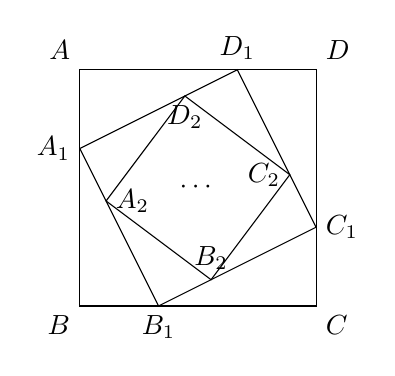
\begin{tikzpicture}
        \draw (0,3) node [above left] {$A$} coordinate (A) -- (0,0) node [below left] {$B$} coordinate (B) -- (3,0) node [below right] {$C$} coordinate (C) -- (3,3) node [above right] {$D$} coordinate (D) -- cycle;
        \draw ($(A)!{1/3}!(B)$) node [left] {$A_1$} coordinate (A1) -- ($(B)!{1/3}!(C)$) node [below] {$B_1$} coordinate (B1) -- ($(C)!{1/3}!(D)$) node [right] {$C_1$} coordinate (C1) -- ($(D)!{1/3}!(A)$) node [above] {$D_1$} coordinate (D1) -- cycle;
        \draw ($(A1)!{1/3}!(B1)$) node [right] {$A_2$} coordinate (A2) -- ($(B1)!{1/3}!(C1)$) node [above] {$B_2$} coordinate (B2) -- ($(C1)!{1/3}!(D1)$) node [left] {$C_2$} coordinate (C2) -- ($(D1)!{1/3}!(A1)$) node [below] {$D_2$} coordinate (D2) -- cycle;
        \draw (1.5,1.5) node {$\cdots$};
    \end{tikzpicture}
\end{center}
\item 如图, 直线$m$: $3x+4y-4=0$与以$O_1,O_2,\cdots, O_n,\cdots$为圆心, 且依次外切的半圆都相切, 其中半圆$O_1$与$y$轴相切, 半圆圆心都在$x$轴的正半轴上, 半径分别为$r_1,r_2,\cdots, r_n,\cdots$, 求所有半圆弧长的总和$L$.
\begin{center}
    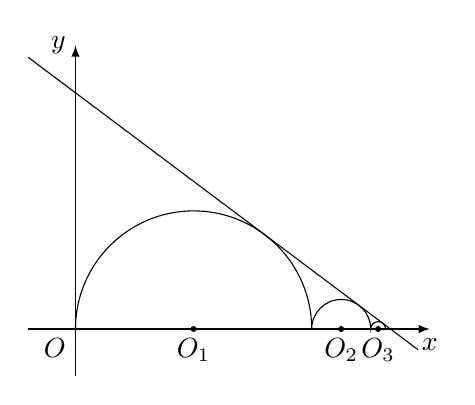
\begin{tikzpicture}[>=latex,scale = 3]
        \draw [->] (-0.2,0) -- (1.5,0) node [below] {$x$};
        \draw [->] (0,-0.2) -- (0,1.2) node [left] {$y$};
        \draw (0,0) node [below left] {$O$};
        \draw [domain = -0.2:1.45] plot (\x,{1-3*\x/4});
        \draw (0,0) arc (180:0:0.5) arc (180:0:{0.5/4}) arc (180:0:{0.5/16});
        \filldraw (0.5,0) circle (0.01) node [below] {$O_1$} (1.125,0) circle (0.01) node [below] {$O_2$} (1.25+0.5/16,0) circle (0.01) node [below] {$O_3$};
    \end{tikzpicture}
\end{center}

\item 从一点$O$顺次引出八条射线$OA,OB,OC,OD,OE,OF,OG,OH$, 其中每相邻两条射线的夹角都是$45^{\circ}$.在$OA$上取$OA=a$, 由$A$作$OB$的垂线$AA_1$, $A_1$是垂足; 由点$A_1$作$OC$的垂线$A_1A_2$, $A_2$是垂足, 由点$A_2$作$OD$的垂线$A_2A_3$, $A_3$是垂足; 然后用同样的方法如此无限继续下去.求所得折线$A_1A_2A_3A_4\cdots$的长度.
\item 已知$S_n=\dfrac 15+\dfrac 2{5^2}+\dfrac 1{5^3}+\dfrac 2{5^4}+\cdots +\dfrac 1{5^{2n-1}}+\dfrac 2{5^{2n}}$($n\in \mathbf{N}^*$), 求$\displaystyle\lim_{n\to\infty}S_n$.
\item 已知无穷等比数列$\{\dfrac 1{2^{n-1}}\cos ^{n-1}\theta\}$的各项和等于$\dfrac 43$, 其中$-\dfrac{\pi }2<\theta <\dfrac{\pi }2$, 求$\theta$的值.
\item 已知正方形的边长为$a$, 作正方形的内切圆, 在此内切圆内作新的内接正方形, 这样一直无限地继续下去.\\
(1) 求所有这些内切圆周长的和;\\
(2) 求所有这些内切圆面积的和.
\item 对于数列$\dfrac 12,\dfrac 14,\cdots ,\dfrac 1{2^n},\cdots$, 试从其中找出无限项构成一个新的等比数列, 使新数列的各项和为$\dfrac 17$, 并求新数列的首项与公比.
\item 已知数列$\{a_n\}$是等差数列, 数列$\{b_n\}$分别满足下列各式, 其中数列$\{b_n\}$必为等差数列的是\bracket{20}.
\fourch{$b_n=|a_n|$}{$b_n=a_n^2$}{$b_n=\dfrac 1{a_n}$}{$b_n=-\dfrac{a_n}2$}
\item 如果数列$\{a_n\}$是一个以$q$为公比的等比数列, $b_n=-2a_n$, 那么数列$\{b_n\}$是  \bracket{20}.
\twoch{以$q$为公比的等比数列}{以$-q$为公比的等比数列}{以$2q$为公比的等比数列}{以$-2q$为公比的等比数列}
\item 在等差数列$\{a_n\}$中, 已知公差$d=\dfrac 12$, 且$a_1+a_3+a_5+\cdots +a_{99}=60$, 求$a_1+a_2+a_3+\cdots +a_{99}+a_{100}$的值.
\item 已知等差数列$\{a_n\}$的前$n$项和为$S_n=t\cdot n^2+(t-9)n+t-\dfrac 32$($t$为常数), 求数列$\{a_n\}$的通项公式.
\item 图中的离散点是$(n,a_n)$的图像, 其中$n\in \mathbf{N}^*$, 如$(1,4)$是第$1$点, 表示$a_1=4$.
\begin{center}
    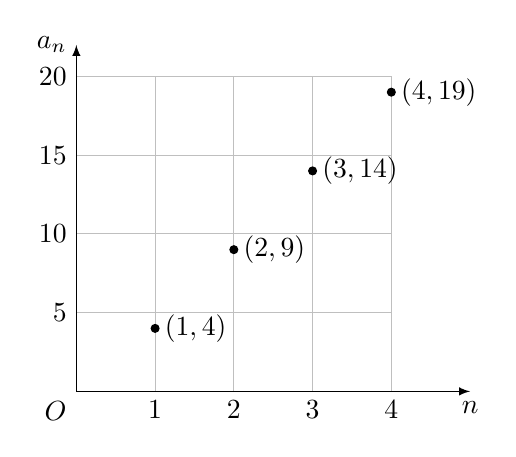
\begin{tikzpicture}[>=latex,yscale = 0.2]
        \foreach \i in {1,2,3,4}
        {
            \draw [gray!50] (\i,0) -- (\i,20);
            \draw [gray!50] (0,{\i*5}) -- (4,{\i*5});
            \filldraw (\i,{5*\i-1}) ellipse (0.05 and 0.25);
            \draw (\i,0) node [below] {$\i$};
        };
        \draw [->] (0,0) -- (5,0) node [below] {$n$};
        \draw [->] (0,0) -- (0,22) node [left] {$a_n$};
        \draw (0,0) node [below left] {$O$};
        \foreach \i in {5,10,15,20}
        {
            \draw (0,\i) node [left] {$\i$};
        };
        \draw (1,4) node [right] {$(1,4)$};
        \draw (2,9) node [right] {$(2,9)$};
        \draw (3,14) node [right] {$(3,14)$};
        \draw (4,19) node [right] {$(4,19)$};
    \end{tikzpicture}
\end{center}
(1) 写出数列$\{a_n\}$的一个通项公式;\\
(2) 计算从第$1$点起的前$46$个点的纵坐标之和.
\item 设$S_n$为等差数列$\{a_n\}$的前$n$项和, 求证: 数列$\{\dfrac{S_n}n\}$是等差数列.
\item 某区域环境噪声平均值如下表:
\begin{center}
    \begin{tabular}{|c|c|c|c|c|}
    \hline
    年份 & $2001$ & $2002$ & $2003$ & $2004$ \\ \hline
    分贝 & $57.8$ & $57.2$ & $56.6$ & $56.0$ \\ \hline
    \end{tabular}
\end{center}
如果噪声平均值按照表中规律依次逐年减小, 那么从哪一年起平均值将小于$42$分贝?
\item 假设某市$2004$年新建住房面积$400$万平方米, 其中有$250$万平方米是中低价房.预计在今后的若干年内, 该市每年新建住房面积平均比上一年增长$8\%$.另外, 每年新建住房中, 中低价房的面积均比上一年增加$50$万平方米.\\
(1) 到哪一年底该市历年所建中低价房的累计面积(以$2004$年为累计的第一年)将首次不少于$4750$万平方米?\\
(2) 到哪一年底当年建造的中低价房的面积占该年建造住房面积的比例首次大于$85\%$?
\item 在用数学归纳法证明等式: $1^2+2^2+\cdots +n^2+\cdots +2^2+1^2=\dfrac{n(2n^2+1)}3$($n\in \mathbf{N}^*$)的过程中, 假设当$n=k$时等式成立后, 在证明当$n=k+1$时等式也成立时, 等式的左边应添加哪些项?
\item 某个命题与正整数有关, 如果当$n=k(k\in \mathbf{N}^*)$时命题成立, 那么可以推得当$n=k+1$时命题也成立.现在已知当$n=5$时该命题不成立, 所以该命题在\bracket{20}.
\fourch{$n=6$时成立}{$n=6$时不成立}{$n=4$时成立}{$n=4$时不成立}
\item 用数学归纳法证明: $\dfrac 12+\dfrac 2{2^2}+\dfrac 3{2^3}+\cdots +\dfrac n{2^n}=2-\dfrac{n+2}{2^n}$($n\in \mathbf{N}^*$).
\item (1) 依次计算下列各式的值:
$\dfrac 11,\dfrac 11+\dfrac 1{1+2},\dfrac 11+\dfrac 1{1+2}+\dfrac 1{1+2+3},\dfrac 11+\dfrac 1{1+2}+\dfrac 1{1+2+3}+\dfrac 1{1+2+3+4}$;\\
(2) 根据第(1)题的计算结果, 猜想$S_n=\dfrac 11+\dfrac 1{1+2}+\dfrac 1{1+2+3}+\cdots +\dfrac 1{1+2+3+\cdots +n}$ ($n\in \mathbf{N}^*$)的表达式, 并用数学归纳法证明你的结论.
\item 若$\displaystyle\lim_{n\to\infty}\dfrac{2^n}{2^{n+1}+a^n}=0$, 则实数$a$的取值范围是\blank{50}.
\item 若$a>0$, 则$\displaystyle\lim_{n\to\infty}\dfrac{3^n-a^n}{3^{n+1}+a^{n+1}}=$\blank{50}.
\item 已知数列$\{a_n\}$是等差数列, 且$a_1\ne 0$, $S_n$为这个数列的前$n$项和.\\
(1) 求$\displaystyle\lim_{n\to\infty}\dfrac{na_n}{S_n}$;\\
(2) 求$\displaystyle\lim_{n\to\infty}\dfrac{S_n+S_{n+1}}{S_n+S_{n-1}}$.
\item 已知等比数列$\{a_n\}$的首项为$1$, 公比为$q(q>0)$, 它的前$n$项和为$S_n$, 且$T_n=\dfrac{S_n}{S_{n+1}}$, 求$\displaystyle\lim_{n\to\infty}T_n$的值.
\item 已知数列$\{\log _3a_n\}$是等差数列, 且$\log _3a_1+\log _3a_2+\cdots +\log _3a_{10}=10$, 求$a_5\cdot a_6$.
\item 在数列$\{a_n\}$中, 设$S_1=a_1+a_2+\cdots +a_n$, $S_2=a_{n+1}+a_{n+2}+\cdots +a_{2n}$, $S_3=a_{2n+1}+a_{2n+2}+\cdots +a_{3n}$.\\
(1) 若数列$\{a_n\}$是等差数列, 求证: 数列$S_1$, $S_2$, $S_3$也是等差数列;\\
(2) 若数列$\{a_n\}$是等比数列, 是否有第(1)题中类似的结论?
\item 已知一个项数有限的等差数列$\{a_n\}$的前$4$项和为$21$, 最后$4$项和为$67$, 这个数列的所有项的和为$286$. 这个数列有多少项?
\item 碘$-131$是一种放射性物质, 在医疗诊断中常会用到它, 下表是$20$克碘$-131$在$4$天内每天衰减的试验数据:\\
\begin{center}
    \begin{tabular}{|c|c|c|c|c|c|}
    \hline
    天数 &	$0$ & $1$ & $2$ & $3$ & $4$ \\ \hline
    剩余克数 & $20.0$ & $18.34$ & $16.82$ & $15.42$ & $14.14$ \\ \hline
    \end{tabular}
\end{center}
$7$天后是否能保证有$10$克该物质用于治疗? 请说明你的理由.
\item 用数学归纳法证明:
$1-\dfrac 12+\dfrac 13-\dfrac 14+\cdots +\dfrac 1{2n-1}-\dfrac 1{2n}=\dfrac 1{n+1}+\dfrac 1{n+2}+\cdots +\dfrac 1{2n}$($n\in \mathbf{N}^*$).
\item 依次计算数列: $(1-\dfrac 14),(1-\dfrac 14)(1-\dfrac 19),(1-\dfrac 14)(1-\dfrac 19)(1-\dfrac 1{16}),(1-\dfrac 14)(1-\dfrac 19)$ $(1-\dfrac 1{16})(1-\dfrac 1{25}),\cdots$的前$4$项的值, 由此猜想$(1-\dfrac 14)(1-\dfrac 19)(1-\dfrac 1{16})(1-\dfrac 1{25})\cdots$ $[1-\dfrac 1{(n+1)^2}]$($n\in \mathbf{N}^*$)的结果, 并用数学归纳法加以证明.
\item 计算: $\displaystyle\lim_{n\to\infty}(\dfrac 1{n^2+1}+\dfrac 2{n^2+1}+\dfrac 3{n^2+1}+\cdots +\dfrac{2k}{n^2+1})$(其中$k$为与$n$无关的正整数).
\item $\displaystyle\lim_{n\to\infty}n^2(\dfrac kn-\dfrac 1{n+1}-\dfrac 1{n+2}-\cdots -\dfrac 1{n+k})$(其中$k$为与$n$无关的正整数).
\item 已知$a=0.4\dot1\dot8$, 若将$a$写成最简分数$\dfrac mn$, 求$n-m$的值.
\item 已知数列$\{a_n\}$是等差数列, $a_1>0$, 且此数列的前$15$项和等于前$20$项和, 求它的前$n$项和的最大值, 并求出此时$n$的值.
\item 已知数列$\{a_n\}$是无穷等比数列, 且公比$q$满足$0<|q|<1$, $a_n=k(a_{n+1}+a_{n+2}+a_{n+3}+\cdots)$, 求实数$k$的取值范围.
\item 是否存在常数$a,b,c$, 使等式$1^2+3^2+5^2+\cdots +(2n-1)^2=\dfrac 13an(bn^2+c)$对任意正整数$n$都成立? 证明你的结论.
\item 已知无穷等比数列$\{a_n\}$的首项为$a$, 公比$q>0$, 设这个数列的前$n$项和为$S_n$, 记$T_n=a_1+a_3+a_5+\cdots +a_{2n-1}$, 求$\displaystyle\lim_{n\to\infty}\dfrac{S_n}{T_n}$的值.
\item 医学上为研究传染病传播中病毒细胞的发展规律及其预防, 将病毒细胞注入一只小白鼠体内进行实验, 经检测, 病毒细胞的增长数与天数的关系记录如下表.已知该种病毒细胞在小白鼠体内的个数超过$10^8$的时候小白鼠将死亡.但注射某种药物, 将可杀死其体内该病毒细胞的$98\%$.
\begin{center}
    \begin{tabular}{|c|c|c|c|c|c|c|c|c|}
        \hline
        天数$t$	& $1$ & $2$ & $3$ & $4$ & $5$ & $6$ & $7$ & $\cdots$ \\ \hline
        病毒细胞总数$N$	& $1$ & $2$ & $4$ & $8$ & $16$ & $32$ & $64$ & $\cdots$ \\ \hline
    \end{tabular}
\end{center}
(1) 为了使小白鼠在实验过程中不死亡, 第一次最迟应在何时注射该种药物(精确到$1$天)?\\
(2) 第二次最迟应在何时注射该种药物, 才能维持小白鼠的生命(精确到$1$天)?
\item 如图所示:
\begin{center}
    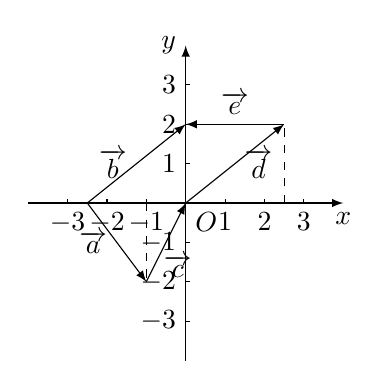
\begin{tikzpicture}[>=latex, scale = 0.5]
        \draw [->] (-4,0) -- (4,0) node [below] {$x$};
        \draw [->] (0,-4) -- (0,4) node [left] {$y$};
        \draw (0,0) node [below right] {$O$};
        \foreach \i in {-3,-2,-1,1,2,3}
        {
            \draw (\i,0.1) -- (\i,0) node [below] {$\i$};
            \draw (0.1,\i) -- (0,\i) node [left] {$\i$};
        };
        \draw [dashed] (2.5,0) -- (2.5,2);
        \draw [->] (2.5,2) -- (0,2); 
        \draw (1.25,2) node [above] {$\overrightarrow e$};
        \draw [->] (0,0) -- (2.5,2);
        \draw (1.25,1) node [right] {$\overrightarrow d$};
        \draw [->] (-2.5,0) -- (0,2);
        \draw (-1.25,1) node [left] {$\overrightarrow b$};
        \draw [->] (-2.5,0) -- (-1,-2);
        \draw (-1.75,-1) node [left] {$\overrightarrow a$};
        \draw [dashed] (-1,0) -- (-1,-2);
        \draw [->] (-1,-2) -- (0,0);
        \draw (-0.8,-1.6) node [right] {$\overrightarrow c$};
    \end{tikzpicture}
\end{center}
(1) 写出向量$\overrightarrow a,\overrightarrow b,\overrightarrow c,\overrightarrow d,\overrightarrow e$的坐标;\\
(2) 找出这些向量中的相等向量;\\
(3) 求$\overrightarrow a-\overrightarrow b+\overrightarrow c+\overrightarrow d+\overrightarrow e$.
\item 用坐标表示下列向量:\\
(1) $-\overrightarrow i$;\\
(2) $2\overrightarrow i+\dfrac 12\overrightarrow j$;\\
(3) 与$x$轴平行且模为$2$的向量;\\
(4) 向东南方向前进$3$个单位的位移.
\item 已知向量$\overrightarrow a=(-3,1)$与$\overrightarrow b=(-1,-3)$.\\
(1) 求$|3\overrightarrow a-\overrightarrow b|$;\\
(2) 求$3\overrightarrow a-\overrightarrow b$的单位向量的坐标.
\item 已知$\overrightarrow a=(x,3)$, $\overrightarrow b=(1,y)$, $\overrightarrow a-2\overrightarrow b=(2,5)$, 求实数$x,y$的值.
\item 已知向量$\overrightarrow a=(2,3)$与$\overrightarrow b=(4,-1+y)$, 且$\overrightarrow a\parallel \overrightarrow b$, 求实数$y$的值.
\item 已知$A,B,C$三点的坐标分别是$(0,1),(1,2),(3,4)$, 求证: $A,B,C$三点共线.
\item 已知$A,B$两点的坐标分别是$(3,-1),(-4,-2)$, $P$是直线$AB$上的点, 根据下列条件求点$P$的坐标:\\
(1) $\overrightarrow{AP}=2\overrightarrow{PB}$;\\
(2) $2\overrightarrow{AP}=3\overrightarrow{BP}$.
\item 在$\triangle ABC$中, 已知$A,B$两点的坐标分别为$(2,1),(-3,4)$, $\triangle ABC$的重心坐标为$(-\dfrac 23,\dfrac 43)$, 求点$C$的坐标.
\item 已知平面上$A,B,C$三点的坐标分别为$(-2,1),(-1,3),(3,4)$, 且$A,B,C,D$这四点构成平行四边形的四个顶点, 求点$D$的坐标.
\item 已知$A,B$两点的坐标分别是$(1,2),(-1,4)$, $\overrightarrow{AC}=\dfrac 12\overrightarrow{AB}$, $\overrightarrow{AD}=2\overrightarrow{CB}$.\\
(1) 求$C,D$的坐标;\\
(2) 求向量$\overrightarrow{BD}$的坐标.
\item 已知$A,B$两点的坐标分别是$(-2,-3),(4,1)$, 延长$AB$到$P$, 使$|\overrightarrow{AP}|=3|\overrightarrow{PB}|$, 求点$P$的坐标.
\item 已知向量$\overrightarrow a=(-2,3)$, 点$A$的坐标是$(2,-1)$, 向量$\overrightarrow{AB}$与$\overrightarrow a$平行, 且$|\overrightarrow{AB}|=2\sqrt {13}$, 求向量$\overrightarrow{OB}$的坐标.
\item 如果$|\overrightarrow a|=2$, $|\overrightarrow b|=\dfrac 12$, $\overrightarrow a$与$\overrightarrow b$的夹角为$60^{\circ }$, 那么$\overrightarrow a$与$\overrightarrow b$的数量积等于\bracket{20}.
\fourch{$\dfrac 12$}{$\dfrac 14$}{$1$}{$2$}
\item 已知$|\overrightarrow b|=3$.如果$\overrightarrow a$在$\overrightarrow b$的方向上的投影是$\dfrac 32$, 那么$\overrightarrow a\cdot \overrightarrow b$为\bracket{20}.
\fourch{$3$}{$\dfrac 92$}{$2$}{$\dfrac 12$}
\item 如果$\overrightarrow a\overrightarrow b$是两个非零向量, 那么``$(\overrightarrow a+\overrightarrow b)^2=\overrightarrow a^2+\overrightarrow b^2$''是``$\overrightarrow a\perp \overrightarrow b$''的\bracket{20}.
\twoch{充分非必要条件}{必要非充分条件}{充要条件}{既非充分又非必要条件}
\item 已知$|\overrightarrow a|=2$, $|\overrightarrow b|=1$.若$\overrightarrow a$与$\overrightarrow b$之间的夹角为$\dfrac{\pi }3$, 则向量$\overrightarrow m=\overrightarrow a-\overrightarrow b$的模为\blank{50}.
\item 在$\triangle ABC$中, 已知$\angle A,\angle B,\angle C$的对边长分别为$a,b,c$. 若$a=3$, $b=1$, $\angle C=30^{\circ}$, 则$\overrightarrow{BC}\cdot \overrightarrow{CA}=$\blank{50}.
\item 若$|\overrightarrow{AB}|=|\overrightarrow{AC}|=6$, $\overrightarrow{AB}\cdot \overrightarrow{AC}=18$, 则$\triangle ABC$的形状是\blank{50}.
\item 已知$|\overrightarrow a|=1$, $|\overrightarrow b|=\sqrt 2$.若$\overrightarrow a-\overrightarrow b$与$\overrightarrow a$垂直, 求$\overrightarrow a$与$\overrightarrow b$的夹角.
\item 已知$|\overrightarrow a|=1$, $|\overrightarrow b|=3$, $|2\overrightarrow a+\overrightarrow b|=\sqrt 7$, 求$\overrightarrow a$与$\overrightarrow b$的夹角.
\item 已知$\overrightarrow a$为非零向量, $\overrightarrow b=(3,4)$, 且$\overrightarrow a\perp \overrightarrow b$, 求$\overrightarrow a$的单位向量$\overrightarrow {a_0}$.
\item 已知向量$\overrightarrow a=(3,4)$与$\overrightarrow b=(5,-12)$, 求$\overrightarrow a\cdot \overrightarrow b$、$|\overrightarrow a-\overrightarrow b|$、$\overrightarrow a$与$\overrightarrow b$的夹角.
\item 已知向量$\overrightarrow a=(3k,3)$与$\overrightarrow b=(-6,k-7)$.\\
(1) 若$\overrightarrow a\perp \overrightarrow b$, 求实数$k$的值;\\
(2) 若$\overrightarrow a\parallel \overrightarrow b$, 求实数$k$的值.
\item 已知向量$\overrightarrow a=(5,12)$与$\overrightarrow b=(4,6)$, 求$\overrightarrow a+\overrightarrow b$与$2\overrightarrow a-3\overrightarrow b$的夹角.
\item 已知$\overrightarrow a+\overrightarrow b+\overrightarrow c=\overrightarrow 0$, 且$|\overrightarrow a|=4$, $|\overrightarrow b|=3$, $|\overrightarrow c|=5$.\\
(1) 求$\overrightarrow a\cdot \overrightarrow c$;\\
(2) 求$\overrightarrow a\cdot \overrightarrow b+\overrightarrow b\cdot \overrightarrow c+\overrightarrow c\cdot \overrightarrow a$.
\item 已知$\overrightarrow a\overrightarrow b$都是非零向量, 且$(\overrightarrow a+3\overrightarrow b)\perp (7\overrightarrow a-5\overrightarrow b)$, $(\overrightarrow a-4\overrightarrow b)\perp (7\overrightarrow a-2\overrightarrow b)$, 求$\overrightarrow a$与$\overrightarrow b$的夹角.
\item 已知位置向量$\overrightarrow a=(2,2)$、$\overrightarrow b=(-3,3)$、$\overrightarrow c=(-1,0)$的终点分别为$A,B,C$, 试判断$\triangle ABC$的形状.
\item 已知向量$\overrightarrow a=(x,2)$与$\overrightarrow b=(-3,-5)$, $\overrightarrow a$与$\overrightarrow b$的夹角为钝角, 求$x$的取值范围.
\item 已知$A,B$两点的坐标分别是$(1,2)$、$(4,-1)$.能否在$y$轴上找到一点$C$, 使$\angle ACB=90^{\circ}$? 若不能, 说明理由; 若能, 求点$C$的坐标.
\item 已知向量$\overrightarrow{OA},\overrightarrow{OB}$, 且点$O,A,B$不共线.
\begin{center}
    \begin{tikzpicture}[>=latex]
        \draw [->] (0,0) node [below] {$O$} -- (135:1) node [left] {$A$};
        \draw [->] (0,0) -- (2,0) node [below] {$B$};
    \end{tikzpicture}
\end{center}
(1)求作向量$\overrightarrow{OM}$, 且$\overrightarrow{OM}=\dfrac 12(\overrightarrow{OA}-\overrightarrow{OB})$;\\
(2)求作向量$\overrightarrow{ON}$, 且$\overrightarrow{ON}=3\overrightarrow{OA}+2\overrightarrow{OB}$.
\item 已知$\overrightarrow a=-\overrightarrow e_1+3\overrightarrow e_2$, $\overrightarrow b=4\overrightarrow e_1+2\overrightarrow e_2$, $\overrightarrow c=-3\overrightarrow e_1+12\overrightarrow e_2$.若以$\overrightarrow b, \overrightarrow c$为一组基, 则$\overrightarrow a$可用$\overrightarrow b,\overrightarrow c$表示为\blank{50}.
\item 如图, 已知$\overrightarrow{OA},\overrightarrow{OB}$不共线, 且$\overrightarrow{AP}=\lambda \overrightarrow{PB}$, 用$\overrightarrow{OA},\overrightarrow{OB}$表示$\overrightarrow{OP}$.
\begin{center}
    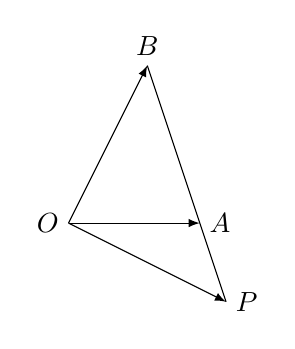
\begin{tikzpicture}[>=latex]
        \draw (0,0) node [left] {$O$} coordinate (O);
        \draw (2,-1) node [right] {$P$} coordinate (P);
        \draw (1,2) node [above] {$B$} coordinate (B);
        \draw ({5/3},0) node [right] {$A$} coordinate (A);
        \draw (B) -- (P);
        \draw [->] (O) -- (A);
        \draw [->] (O) -- (B);
        \draw [->] (O) -- (P);
    \end{tikzpicture}
\end{center}
\item 在$\triangle ABC$中, 已知$\overrightarrow{AB}=\overrightarrow a$, $\overrightarrow{AC}=\overrightarrow b$, 且$\overrightarrow{AD}=\dfrac 12\overrightarrow{AB}$, $\overrightarrow{AE}=\dfrac 12\overrightarrow{AC}$.求证: $\overrightarrow{DE}=\dfrac 12\overrightarrow{BC}$.
\item 在矩形$ABCD$中, $\overrightarrow{AB}=\overrightarrow a$, $\overrightarrow{AD}=\overrightarrow b$, $E,F,G,H$分别是边$AB,BC,CD,DA$的中点, 用$\overrightarrow a,\overrightarrow b$分别表示$\overrightarrow{EF},\overrightarrow{EH},\overrightarrow{FG}$, 并指出$\overrightarrow{EH}$与$\overrightarrow{FG}$的关系.
\item 如图, 已知$|\overrightarrow{OA}|=|\overrightarrow{OB}|=1$, $\overrightarrow{OA}$与$\overrightarrow{OB}$的夹角为$120^{\circ }$, $\overrightarrow{OC}$与$\overrightarrow{OA}$的夹角为$25^{\circ }$, $|\overrightarrow{OC}|=2\sqrt 3$, 用$\overrightarrow{OA},\overrightarrow{OB}$表示$\overrightarrow{OC}$.
\begin{center}
    \begin{tikzpicture}[>=latex]
        \draw (0,0) node [below] {$O$} coordinate (O);
        \draw (1,0) node [below] {$A$} coordinate (A);
        \draw (120:1) node [left] {$B$} coordinate (B);
        \draw (25:{2*sqrt(3)}) node [above] {$C$} coordinate (C);
        \draw [->] (O) -- (A);
        \draw [->] (O) -- (B);
        \draw [->] (O) -- (C);
    \end{tikzpicture}
\end{center}
\item 如图, 已知$ED$分别是$\triangle ABC$中$AC, BC$边上的点, 且$AE=2EC$, $BD=\dfrac 13BC$.若$\overrightarrow{AB}=\overrightarrow a$, $\overrightarrow{BC}=\overrightarrow b$, 试用$\overrightarrow a, \overrightarrow b$表示$\overrightarrow{ED}$.
\begin{center}
    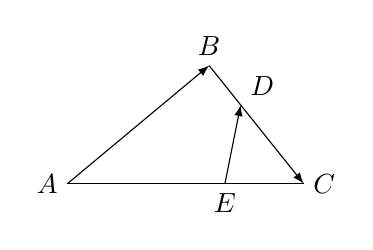
\begin{tikzpicture}[>=latex]
        \draw (0,0) node [left] {$A$} coordinate (A);
        \draw (2,0) node [below] {$E$} coordinate (E);
        \draw (3,0) node [right] {$C$} coordinate (C);
        \draw (2.2,1) node [above right] {$D$} coordinate (D);
        \draw (1.8,1.5) node [above] {$B$} coordinate (B);
        \draw (A) -- (C);
        \draw [->] (E) -- (D);
        \draw [->] (A) -- (B);
        \draw [->] (B) -- (C);
    \end{tikzpicture}
\end{center}
\item 如图, 已知四边形$OACB$是平行四边形, 向量$\overrightarrow{OA}=\overrightarrow a$, $\overrightarrow{OB}=\overrightarrow b$, $BM=MN=\dfrac 13BA$, 试用$\overrightarrow a,\overrightarrow b$表示$\overrightarrow{MC},\overrightarrow{ON}$.
\begin{center}
    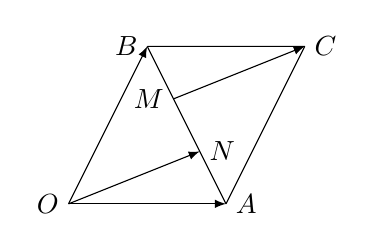
\begin{tikzpicture}[>=latex]
        \draw (0,0) node [left] {$O$} coordinate (O);
        \draw (2,0) node [right] {$A$} coordinate (A);
        \draw (1,2) node [left] {$B$} coordinate (B);
        \draw (3,2) node [right] {$C$} coordinate (C);
        \draw ($(A)!{1/3}!(B)$) node [right] {$N$} coordinate (N);
        \draw ($(A)!{2/3}!(B)$) node [left] {$M$} coordinate (M);
        \draw (A) -- (B) (A) -- (C) (B) -- (C);
        \draw [->] (O) -- (A);
        \draw [->] (O) -- (N);
        \draw [->] (O) -- (B);
        \draw [->] (M) -- (C);

    \end{tikzpicture}
\end{center}
\item 用向量法证明: 对角线相等的平行四边形是矩形.
\item 在直角三角形$ACB$中, $AD$是斜边$BC$上的高, 用向量法证明: $AD^2=BD\cdot DC$.
\item 已知$xy\in \mathbf{R}$, 用向量法证明$x^2+y^2\ge 2xy$.
\item 如果某超市的商品甲乙两种商品的单价分别为$a,b$, 那么$(a,b)$叫做该两种商品的价格向量; 如果某一天超市卖出甲乙两种商品数量分别为$x,y$, 那么$(x,y)$叫做这两种商品的销售向量.试解释价格向量与销售向量的数量积的意义.
\item 已知三个力$\overrightarrow{f_1}$、$\overrightarrow{f_2}$和$\overrightarrow{f_3}$作用于同一质点, 且$|\overrightarrow{f_1}|=20$, $|\overrightarrow{f_2}|=30$, $|\overrightarrow{f_3}|=40$(单位: 牛).若三个力的夹角都为$120^{\circ }$, 求合力的大小和方向.
\begin{center}
    \begin{tikzpicture}[>=latex,scale = 0.4]
        \draw [->] (0,0) -- (240:2) node [below] {$\overrightarrow {f_1}$};
        \draw [->] (0,0) -- (120:3) node [above] {$\overrightarrow {f_2}$};
        \draw [->] (0,0) -- (0:4) node [right] {$\overrightarrow {f_3}$};
    \end{tikzpicture}
\end{center}
\item 在直角三角形$CAB$中, $AD$是斜边$BC$上的中线, 用向量法证明: $|\overrightarrow{AD}|=\dfrac 12|\overrightarrow{BC}|$.
\item 已知$\overrightarrow{OA},\overrightarrow{OB}$不共线, 点$P$在$OAB$所在平面内, 且$\overrightarrow{OP}=(1-t)\overrightarrow{OA}+t\overrightarrow{OB}$($t\in \mathbf{R}$).求证: $A,B,P$三点共线.
\item 如图, 有一个质量为$4$千克的匀质球, 它的半径$R$为$6$厘米.将这个球放在墙与均匀的木板$AB$之间, $A$端固定在墙上, $B$端用水平绳索$BC$拉住, 板长$AB$为$40$厘米.如果木板的质量忽略不计, 当$\alpha$为$60^{\circ }$时, 求绳的拉力.(精确到$1$牛)
\begin{center}
    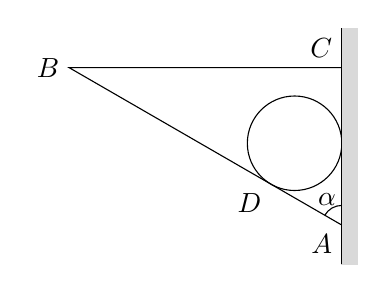
\begin{tikzpicture}[scale = 0.1]
        \draw (0,0) node [below left] {$A$} coordinate (A);
        \draw (150:40) node [left] {$B$} coordinate (B);
        \draw (0,20) node [above left] {$C$} coordinate (C);
        \draw (A) -- (B) -- (C);
        \draw (120:12) circle (6);
        \draw (150:{6*sqrt(3)}) node [below left] {$D$};
        \draw (A) pic ["$\alpha$", draw, scale = 0.5, angle eccentricity = 1.5] {angle = C--A--B};
        \filldraw [gray!30] (0,-5) rectangle (2,25);
        \draw (0,-5) -- (0,25);
    \end{tikzpicture}
\end{center}
\item 在平行四边形$ABCD$中, $AB=1$, $AD=2$, $\angle DAB=60^{\circ }$, 求对角线$AC$与$BD$的夹角.
*****
\item 已知$MN$两点的坐标分别是$(3,-2)$、$(-5,-1)$, 且$\overrightarrow{MP}=\overrightarrow{PN}$, 求点$P$的坐标.
\item 已知平面内三个点$ABC$的坐标分别是$(-1,2)$、$(10,-1)$、$(-4,3)$, $G$是已知平面内的一点, 且$\overrightarrow{AG}+\overrightarrow{BG}+\overrightarrow{CG}=\overrightarrow 0$, 求点$G$的坐标.
\item 已知向量$\overrightarrow a=(3,4)$与$\overrightarrow b=(1,0)$.
(1)求$\overrightarrow a$在$\overrightarrow b$的方向上的投影.
(2)求$\overrightarrow b$在$\overrightarrow a$的方向上的投影.
\item 已知$|\overrightarrow{AB}|=2$, $|\overrightarrow{AC}|=4$, $|\overrightarrow{AB}-\overrightarrow{AC}|=2\sqrt 3$, 求$\overrightarrow{AB}$与$\overrightarrow{AC}$的夹角.
\item 以原点$O$和点$A(5,2)$为顶点作等腰直角三角形$ABO$, 使$\angle B=90^{\circ }$, 求向量$\overrightarrow{OB}$的坐标.
\item 已知$ABD$的坐标分别是$(0,-1)$、$(-5,1)$、$(7,2)$, 且$\overrightarrow{DC}\parallel \overrightarrow{AB}$, $\overrightarrow{BC}\perp \overrightarrow{AB}$, 求点$C$的坐标.
\item 如图, $AMB$在同一直线上, 且$\overrightarrow{AM}=\dfrac 13\overrightarrow{AB}$, 设$\overrightarrow{OA}=\overrightarrow a$, $\overrightarrow{OB}=\overrightarrow b$, $\overrightarrow{OM}=\overrightarrow c$, 用$\overrightarrow a$、$\overrightarrow b$表示$\overrightarrow c$.
(第7题)
\item 已知物体在力$\overrightarrow{f_1}$和$\overrightarrow{f_2}$的作用下从$A(3,-5)$移动到$B(-1,2)$(单位: 米), 且$\overrightarrow{f_1}=2\overrightarrow i-3\overrightarrow j$, $\overrightarrow{f_2}=\overrightarrow i+7\overrightarrow j$(单位: 牛), 求$\overrightarrow{f_1}$与$\overrightarrow{f_2}$的合力$\overrightarrow F$对物体所作的功$W$.
\item 已知$\overrightarrow{e_1}$与$\overrightarrow{e_2}$是不平行的两个向量, 实数$xy$满足: $3x\overrightarrow{e_1}+(10-y)\overrightarrow{e_2}=(4y+7)\overrightarrow{e_1}+2x\overrightarrow{e_2}$, 求$5x-3y$.
\item 已知$\overrightarrow{OP}=(\cos \theta ,\sin \theta)$, $\overrightarrow{OQ}=(1+\sin \theta ,1+\cos \theta)$, 且$0\le \theta \le \pi$.
(1)求$|\overrightarrow{PQ}|$的最大值, 并指出$|\overrightarrow{PQ}|$取最大值时$\theta$的值.
(2)当$|\overrightarrow{PQ}|$取最大值时, 求$\overrightarrow{OP}$与$\overrightarrow{OQ}$的夹角.
\item 如图, 用两根绳子把质量为$10$千克的物体$W$吊在水平杆子$AB$上, $\angle ACW=150^{\circ }$, $\angle BCW=120^{\circ }$, 如果绳子的质量忽略不计, 求$A$处和$B$处所受力的大小.
(第11题)
复 习 题
B组
\item 已知$\overrightarrow a$、$\overrightarrow b$都是非零向量, 且$|\overrightarrow a|=|\overrightarrow b|=|\overrightarrow a-\overrightarrow b|$, 求$\overrightarrow a$与$\overrightarrow a+\overrightarrow b$的夹角.
\item 已知$x\overrightarrow a+3\overrightarrow b=\overrightarrow c$, $\overrightarrow a=(2x,\dfrac 23)$, $\overrightarrow b=(x,y)$, $\overrightarrow c=(-1,\dfrac 83)$, 求实数$xy$的值.
\item 已知$\overrightarrow a$、$\overrightarrow b$、$\overrightarrow c$都是非零向量, 其中任意两个向量都不平行, 已知$\overrightarrow a+\overrightarrow b$与$\overrightarrow c$平行, $\overrightarrow a+\overrightarrow c$与$\overrightarrow b$平行, 求证: $\overrightarrow b+\overrightarrow c$与$\overrightarrow a$平行.
\item 已知两个非零向量$\overrightarrow a$、$\overrightarrow b$, 且$\overrightarrow a\parallel \overrightarrow b$, $|\overrightarrow a|=2$, $|\overrightarrow b|=1$, 求$|\overrightarrow a+t\overrightarrow b|$取最小值时实数$t$的值.
\item 已知$\overrightarrow a=(1,-2)$, $\overrightarrow b=(2,3)$, $\overrightarrow c=(1,1)$, 将$\overrightarrow a$表示成$\overrightarrow b_1+\overrightarrow c_1$的形式, 其中$\overrightarrow b_1\parallel \overrightarrow b$, $\overrightarrow c_1\parallel \overrightarrow c$.
\item 如图, $|\overrightarrow{OA}|=|\overrightarrow{AB}|=|\overrightarrow{BC}|=1$, $\theta \in (0,\dfrac{\pi }2)$, 试用$\theta$表示点$C$的坐标.
(第6题)
\item 如图, 物体$W$的质量为$50$千克, 用绳子将物体$W$悬挂在两面墙之间.已知两面墙之间的距离$AB$为$10$米($AB$为水平线), $AC$为$6$米, $BC$为$8$米, 求$ACBC$上所受的力的大小.(精确到$1$牛)
(第7题)
\item 假设某班的男生中, 步行上学、骑自行车上学和乘车上学的人数分别为$12$、$5$、$3$, 而在这个班的女生中, 采取相应方式上学的人数分别为$10$、$3$、$7$, 试设计一个矩阵来表示这些数据.
\item 已知矩阵$A=\begin{pmatrix}
    1  x  \\y  -1  \end{pmatrix}$和$B=\begin{pmatrix}
    m  0  \\-1  n  \end{pmatrix}$.当$A=B$时, 求实数$xymn$的值.
\item 写出下列线性方程组的系数矩阵和增广矩阵, 并用矩阵变换的方法求解.
(1)$\begin{cases}
    2x+y=5,  \\3x-2y=4.  \end{cases}$ (2)$\begin{cases}
    x+y+z=6,  \\3x+y-z=2,  \\5x-2y+3z=10.  \end{cases}$
\item 利用网络, 查出北京、天津、上海和重庆四个直辖市之间的距离(单位: 千米), 并用矩阵表示.
\item 写出下列线性方程组的系数矩阵和增广矩阵, 并用矩阵变换的方法求解.
(1)$\begin{cases}
    x-2y=3,  \\2x+y=11.  \end{cases}$ (2)$\begin{cases}
    x-2z=1,  \\y+4z=6,  \\2x-y+z=5.  \end{cases}$
\item 填空:
(1)$\begin{pmatrix}
    1  2  \\-1  -1  \end{pmatrix}+\begin{pmatrix}
    -1  2  \\2  1  \end{pmatrix}=$\blank{50}.
(2)$2\begin{pmatrix}
    0  1  \\1  0  \end{pmatrix}-3\begin{pmatrix}
    1  0  \\0  1  \end{pmatrix}=$\blank{50}.
\item 已知$A=\begin{pmatrix}
    0  1  2  \\-1  2  0  \end{pmatrix}$, $B=\begin{pmatrix}
    3  0  3  \\0  -2  5  \end{pmatrix}$.
(1)求$A+B$.
(2)求$B-A$.
(3)求$3A$.
\item 计算下列矩阵的乘积:
(1)$\begin{pmatrix}
    x  y  \\u  v  \end{pmatrix}\begin{pmatrix}
    -1  0  \\0  1  \end{pmatrix}$. (2)$\begin{pmatrix}
    0  0  1  \\1  0  0  \\0  1  0  \end{pmatrix}\begin{pmatrix}
    a  b  c  \\u  v  w  \\x  y  z  \end{pmatrix}$.
(3)$\begin{pmatrix}
    1  2  3  4  \end{pmatrix}\begin{pmatrix}
    1  \\2  \\3  \\4  \end{pmatrix}$.
\item 已知矩阵$A=\begin{pmatrix}
    1  1  \\1  1  \end{pmatrix}$, 求向量$(2,3)$经过矩阵$A$变换后所得的向量.
\item 某水果批发部向$ABCD$四家水果店分别批发的苹果、橘子和香蕉的数量如下(单位: 千克):
苹果	橘子	香蕉
水果店$A$	100	40	60
水果店$B$	60	35	50
水果店$C$	60	30	60
水果店$D$	50	45	30
已知苹果、橘子和香蕉的批发价分别为每千克$1.50$元、$1.80$元和$2.20$元.
(1)试用矩阵表示批发部批发苹果、橘子和香蕉各为多少千克?
(2)试用矩阵表示并计算, $ABCD$四家水果店应支付的金额各为多少元?
\item 在一次演讲比赛中, 如果规定评综合得分的指标有三项: 演说词、口才和仪态, 它们的权重依次为$50\%$、$30\%$和$20\%$, 现有$5$位演讲者的得分如下:
演说词	口才	仪态
演讲者1	90	90	90
演讲者2	90	85	80
演讲者3	80	85	90
演讲者4	80	60	50
演讲者5	50	60	80
试根据三项指标的权重, 用矩阵表示并计算$5$位演讲者的综合得分.
\item 已知矩阵$A=\begin{pmatrix}
    3  1  4  \\2  -1  -2  \\2  4  1  \end{pmatrix}$与$B=\begin{pmatrix}
    0  1  2  \\3  4  -1  \\-2  1  1  \end{pmatrix}$, 求$2A+3B$和$5A-2B$.
\item 已知矩阵$A=\begin{pmatrix}
    5  8  \\6  7  \end{pmatrix}$, 矩阵$B=\begin{pmatrix}
    5  3  4  \\2  2  4  \end{pmatrix}$, 矩阵$C=\begin{pmatrix}
    15  \\10  \\6  \end{pmatrix}$.
(1)求$AB$. (2)求$(AB)C$.
(3)求$BC$. (4)求$A(BC)$.
\item 计算:
(1)$(\begin{pmatrix}
    1  0  \\0  1  \end{pmatrix}-2\begin{pmatrix}
    0  1  \\1  0  \end{pmatrix})\begin{pmatrix}
    1  -1  \\-1  1  \end{pmatrix}$.
(2)$(\begin{pmatrix}
    1  2  \\-2  3  \\3  -5  \end{pmatrix}+\begin{pmatrix}
    2  3  \\2  4  \\-1  0  \end{pmatrix})\begin{pmatrix}
    2  -1  \\1  3  \end{pmatrix}$.
\item 已知向量$(x,y)$经矩阵$\begin{pmatrix}
    0  1  \\1  0  \end{pmatrix}$变换后得到矩阵$(3,2)$, 求实数$xy$的值.
\item 一家水果店共出售五种水果, 它们的单价和利润如下表所示(单位: 元/千克):
品  种	西瓜	哈密瓜	芒果	葡萄	草莓
单价	3.00	6.50	4.50	5.00	8.00
利润	0.50	1.50	1.00	1.20	1.30
该家水果店的经理要在计算每笔生意营业额的同时, 获知该笔生意的利润额.假设现有$3$位顾客来购买水果, 他们的购买量如下表所示(单位: 千克):
西瓜	哈密瓜	芒果	葡萄	草莓
顾客甲	10	5	8.5	3	2
顾客乙	0	15	5	2.5	5
顾客丙	15	10	10	8	7.5
计算每笔生意的营业额和利润.(精确到$0.01$元)
\item 填空:
如果$\begin{vmatrix}
    5  3  \\2  4  \end{vmatrix}+\begin{vmatrix}
    a  -1  \\1  b  \end{vmatrix}=\begin{vmatrix}
    1  2  \\7  8  \end{vmatrix}$, 那么$ab$可以分别取\blank{50}(只需填写$2$组即可).
\item 计算下列行列式的值:
(1)$\begin{vmatrix}
    -6  -2  \\8  5  \end{vmatrix}$. (2)$\begin{vmatrix}
    \sqrt 3-\sqrt 2  \sqrt 3-2  \\\sqrt 3+2  \sqrt 3+\sqrt 2  \end{vmatrix}$.
(3)$\begin{vmatrix}
    \pi ^{m+n}  \pi ^m-1  \\\pi ^m+1  \pi ^{m-n}  \end{vmatrix}$.
\item 用行列式解下列方程组:
(1)$\begin{matrix}
    x+2y=3,  \\4x-y=3.  \end{matrix}$ (2)$\begin{matrix}
    7x-5y-6=0,  \\13x+9y-2=0.  \end{matrix}$
\item 判别下列二元一次方程组解的情况:
(1)$\begin{cases}
    2x-3y=7,  \\3x-4y=11.  \end{cases}$ (2)$\begin{cases}
    x-3y=2,  \\3x-9y=6.  \end{cases}$
(3)$\begin{cases}
    2x+3y=1,  \\4x+6y=3.  \end{cases}$
\item 解下列关于$xy$的方程组:
(1)$\begin{cases}
    x\cos \theta -y\sin \theta =\sin \theta ,  \\x\sin \theta +y\cos \theta =\cos \theta .  \end{cases}$
(2)$\begin{cases}
 (a+b)x+(a-b)y=a^2-b^2,  \\(a-b)x+(a+b)y=a^2+b^2.  \end{cases} (ab\ne 0)$
\item 解关于$xy$的方程组$\begin{cases}
    mx+y=m+1,  \\x+my=2m,  \end{cases}$并对解的情况进行讨论.
\item 已知关于$xy$的方程组$\begin{cases}
 (a^2-2)x-(a+1)y=a+1,  \\a^2x-(a+1)y=a-1  \end{cases}$有唯一解, 求$a$的取值范围.
\item 展开下列行列式并化简:
(1)$\begin{vmatrix}
    x-1  x^2  \\1  x+1  \end{vmatrix}$. (2)$\begin{vmatrix}
    \mathrm{e}^x  \mathrm{e}^x-1  \\\mathrm{e}^x+1  \mathrm{e}^{-x}  \end{vmatrix}$.
\item 用行列式解下列方程组:
(1)$\begin{matrix}
    15x-7y+5=0,  \\22x-6y-14=0.  \end{matrix}$ (2)$\begin{cases}
    \dfrac 5x+\dfrac 7y=3,  \\\dfrac 7x+\dfrac 9y=4.  \end{cases}$
\item 判别下列二元一次方程组解的情况:
(1)$\begin{cases}
    x\cdot \sin ^275^{\circ }+y\cdot \cos ^275^{\circ }=1,  \\x\cdot \sin ^215^{\circ }+y\cdot \cos ^215^{\circ }=2.  \end{cases}$ (2)$\begin{cases}
    2x+y\cdot \lg 2=4,  \\4x+y\cdot \lg 4=8.  \end{cases}$
\item 编出二元一次方程组, 分别满足下列条件.
(1)方程组有唯一解.
(2)方程组无解.
(3)方程组有无穷多解.
\item 计算下列行列式的值: $\begin{vmatrix}
    a  b  \\c  d  \end{vmatrix}$、$\begin{vmatrix}
    a  a+b  \\c  c+d  \end{vmatrix}$.你能得到关于行列式的一个怎样的性质? 猜想行列式还可能具有哪些类似的性质, 并加以证明.
\item 用对角线法则计算下列三阶行列式:
(1)$\begin{vmatrix}
    2  1  2  \\-3  4  -1  \\3  6  5  \end{vmatrix}$. (2)$\begin{vmatrix}
    1  -2  0  \\2  1  0  \\6  3  1  \end{vmatrix}$.
\item 用对角线法则展开下列三阶行列式, 并化简:
(1)$\begin{vmatrix}
    a  b  a+b  \\b  a+b  a  \\a+b  a  b  \end{vmatrix}$. (2)$\begin{vmatrix}
    0  x  y  \\x  0  z  \\y  z  0  \end{vmatrix}$.
\item 试根据三阶行列式的展开式的定义, 将三阶行列式$\begin{vmatrix}
    a_1  b_1  c_1  \\a_2  b_2  c_2  \\a_3  b_3  c_3  \end{vmatrix}$推导成按第二列展开的形式.
\item 用按某一行(或某一列)展开的方式计算下列三阶行列式:
(1)$\begin{vmatrix}
    1  2  2  \\0  3  1  \\2  0  5  \end{vmatrix}$. (2)$\begin{vmatrix}
    1  0  2  \\-3  4  -1  \\2  0  5  \end{vmatrix}$.
\item 用按某一行(或某一列)展开的方式化简下列三阶行列式:
(1)$\begin{vmatrix}
    x  y  z  \\y  x  y  \\z  z  x  \end{vmatrix}$. (2)$\begin{vmatrix}
    0  0  a  \\0  b  c  \\c  a  b  \end{vmatrix}$.
\item 把$\begin{vmatrix}
    x_2  y_2  \\x_3  y_3  \end{vmatrix}-\begin{vmatrix}
    x_1  y_1  \\x_3  y_3  \end{vmatrix}+\begin{vmatrix}
    x_1  y_1  \\x_2  y_2  \end{vmatrix}$表示成一个三阶行列式.
\item 用行列式解下列三元一次方程组:
(1)$\begin{cases}
    x-2y+z=7,  \\3x-5y+z=14,  \\2x-2y-z=3.  \end{cases}$ (2)$\begin{cases}
    x+3y+z=11,  \\2x+3y-4z=13,  \\-x-3y+z=-9.  \end{cases}$
\item 用行列式解关于$xyz$的方程组$\begin{cases}
    x+y=a,  \\y+z=b,  \\z+x=c.  \end{cases}$
\item 当实数$ab$为何值时, 关于$xyz$的方程组$\begin{cases}
    ax+y+z=1,  \\ax+by+z=2,  \\x+2by+z=4  \end{cases}$有唯一解?
\item 某工厂今年$1$月、$2$月、$3$月生产某种产品的数量分别为$1$万件、$1.2$万件、$1.3$万件.为了估计以后每个月的产量, 以这三个月的产品数量为依据, 可用一个二次函数来拟合该产品的月产量$y$(万件)与月份数$x$之间的关系.试求这个二次函数的表达式, 并估算出$4$月份的产量.
\item 填空:
(1)把$3\begin{vmatrix}
    1  3  \\3  1  \end{vmatrix}-2\begin{vmatrix}
    0  -2  \\3  1  \end{vmatrix}-2\begin{vmatrix}
    0  -2  \\1  3  \end{vmatrix}$表示成一个三阶行列式为\blank{50}.
(2)对于方程组\fourch{$\begin{cases}
    a_1x+b_1y+c_1z=d_1,  \\a_2x+b_2y+c_2z=d_2,  \\a_3x+b_3y+c_3z=d_3,  \end{cases}$若记$D=\begin{vmatrix}
    a_1  b_1  c_1  \\a_2  b_2  c_2  \\a_3  b_3  c_3  \end{vmatrix}$, 则``$D=0$''是``方程组(A)有无穷多解''的\blank{50}条件.
\item 用行列式解关于$xyz$的方程组$\begin{cases}
    x-y+z=a,  \\x+y-z=b,  \\-x+y+z=c.  \end{cases}$
\item 已知二次函数$f(x)=ax^2+bx+c$满足$f(1)=0$, $f(2)=3$, $f(-3)=28$, 求$abc$的值.
\item 已知甲、乙、丙三种化肥, 每千克化肥中氮、磷、钾的含量如下表(单位: 克):
氮	磷	钾
甲	70	8	2
乙	64	10	0.6
丙	70	5	1.4
如果要配制$23$千克的混合化肥, 且含磷$149$克、钾$30$克, 那么需要这三种化肥各多少千克?
复 习 题
A组
\item 已知某个线性方程组的增广矩阵是$\begin{pmatrix}
    6  -4  5  \\8  -3  2  \end{pmatrix}$.
(1)试写出这个增广矩阵对应的线性方程组.
(2)用矩阵变换的方法解这个方程组.
\item 已知矩阵$A=\begin{pmatrix}
    2  1  \\-4  0  \end{pmatrix}$, 矩阵$B=\begin{pmatrix}
    4  3  \\-7  0  \end{pmatrix}$, 矩阵$C=\begin{pmatrix}
    1  -2  0  \\-2  3  4  \end{pmatrix}$.
(1)求$B-2A$. (2)求$AB$.
(3)求$AC$.
\item 填空:
(1)两角差的余弦公式为: $\cos (\alpha -\beta)=\cos \alpha \cos \beta +\sin \alpha \sin \beta$, 右式若用行列式表示, 则$\cos (\alpha -\beta)=$\blank{50}.
(2)对于方程组(A)$\begin{cases}
    a_1x+b_1y=c_1,  \\a_2x+b_2y=c_2,  \end{cases}$若记$D=\begin{vmatrix}
    a_1  b_1  \\a_2  b_2  \end{vmatrix}$, $D_x=\begin{vmatrix}
    c_1  b_1  \\c_2  b_2  \end{vmatrix}$, $D_y=\begin{vmatrix}
    a_1  c_1  \\a_2  c_2  \end{vmatrix}$, 则``方程组(A)无解''的充要条件是\blank{50}.
\item 计算下列行列式:
(1)$\begin{vmatrix}
    3+\sqrt 5  \sqrt 3-2  \\\sqrt 3+2  3-\sqrt 5  \end{vmatrix}$. (2)$\begin{vmatrix}
    3  3  -5  \\0  -2  1  \\7  1  3  \end{vmatrix}$.
\item 利用行列式解下列方程组:
(1)$\begin{cases}
    2x-10y=3,  \\4x+5y=1.  \end{cases}$ (2)$\begin{cases}
    3x+2y+z=3,  \\-7x+4y+5z=-10,  \\2x+3y-z=\dfrac 92.  \end{cases}$
(3)$\begin{cases}
    \dfrac{11}x-\dfrac 1y-6=0,  \\\dfrac 3x+\dfrac 5y+1=0.  \end{cases}$
\item 解关于$xy$的方程组$\begin{cases}
    mx+2y=8,  \\2x+(m-3)y=m,  \end{cases}$并对解的情况进行讨论.
\item 当$a$为何值时, 关于$xyz$的方程组$\begin{cases}
    ax+y+z=1,  \\x+ay+z=2,  \\3x+(2a+1)y+3z=6  \end{cases}$有唯一解?
\item 甲、乙、丙三人参与完成一项工作, 若甲乙两人合作, 则甲做$8$天, 乙做$5$天能够完成工作; 若甲丙两人合作, 则甲做$6$天, 丙做$9$天能够完成工作; 若乙丙两人合作, 则乙做$10$天, 丙做$6$天能够完成工作.若这项工作分别由甲、乙、丙单独做, 则他们各需多少天才能完成这项工作?
复 习 题
B组
\item 已知矩阵$A=\begin{pmatrix}
    2  \\1  \\-3  \end{pmatrix}$, 矩阵$B=(\begin{cases}
    -1  2  \end{cases})$, 矩阵$C=\begin{pmatrix}
    -3  0  \\-1  2  \end{pmatrix}$, 求$(AB)C$和$A(BC)$.
\item 填空:
关于$xyz$的方程组$\begin{cases}
    ay+bz=c,  \\cx+az=b,  \\bx+cy=a  \end{cases}$有唯一解的条件是\blank{50}.
\item 用行列式解关于$xyz$的方程组:
$\begin{cases}
    bx-ay=-2ab,  \\-2cy+3bz=bc,(abc\ne 0)  \\cx+az=0.  \end{cases}$
\item 用行列式解关于$xy$的方程组:
$\begin{cases}
 (m-1)x-y-m-1=0,  \\(m-1)x+(m+1)y+1=0.  \end{cases}$
\item 已知关于$xy$的方程组$\begin{cases}
    kx-y=5,  \\2x+3ky=7  \end{cases}$的解满足条件$x>0$, $y<0$, 求实数$k$的取值范围.
总复习题
A组
\item 填空:
(1)数列$-\dfrac 32,\dfrac 54,-\dfrac 76,\dfrac 98,\cdots$的一个通项公式为\blank{50}.
(2)用数学归纳法证明$2+3+4+\cdots +n=\dfrac{(n-1)(n+2)}2$时, 第(i)步取
$n=$\blank{50}验证.
(3)$\displaystyle\lim_{n\to\infty}\dfrac{1+(-1)^n}n=$\blank{50}.
(4)已知向量$\overrightarrow a=(1,2)$与$\overrightarrow b=(3,-2)$.当$k=$\blank{50}时, $k\overrightarrow a+\overrightarrow b$与$\overrightarrow a-3\overrightarrow b$垂直.
\item 选择题:
(1)数列$27, 207, 2 007, 20 007$的一个通项公式可以为\bracket{20}.
(A)$a_n=2n+7$}{$a_n=2^n+7$}{$a_n=20^n+7$}{$a_n=2\times 10^n+7$}
(2)某厂去年的产值是$100$万元, 计划今后$3$年内每年的产值都比上一年增加$10\%$, 从今年起这$3$年的总产值为(精确到$1$万元)\bracket{20}.
\fourch{$121$万元}{约$133$万元}{$331$万元}{约$364$万元}
(3)用数学归纳法证明: $f(n)=1+\dfrac 12+\dfrac 13+\cdots +\dfrac 1{2^n}$($n\in \mathbf{N}^*$)的过程中, 从$n=k$到$n=k+1$时, $f(k+1)$比$f(k)$共增加了\bracket{20}.
\fourch{1项}{$2^k-1$项}{$2^{k+1}$项}{$2^k$项}
(4)在$\triangle ABC$中, 已知$\overrightarrow{AB}=\overrightarrow a$, $\overrightarrow{AC}=\overrightarrow b$, 当$\overrightarrow a\cdot \overrightarrow b<0$时, $\triangle ABC$为\bracket{20}.
\fourch{钝角三角形}{直角三角形}{锐角三角形}{等腰直角三角形}
\item 已知数列$\{a_n\}$的通项公式, 分别写出数列的前$4$项.
(1)$a_n=(-1)^{n+1}\dfrac{3n-1}{n^2+1}$.
(2)$a_n=\begin{cases}
    \cos \dfrac{n\pi }4 (n=2k-1,k\in \mathbf{N}^*),  \\2^n+\dfrac 1{n+1} (n=2k,k\in \mathbf{N}^*).  \end{cases}$
\item 已知数列$\{a_n\}$和数列$\{b_n\}$都是等差数列, $c_n=2\times 3^{a_n+2b_n}$, 求证: 数列$\{c_n\}$是等比数列.
\item 一个水池有若干个流量相同的水龙头, 如果所有水龙头同时放水, 那么$24$小时可以注满水池. 如果开始时水龙头全部开放, 以后每隔相等的时间关闭$1$个水龙头, 到最后$1$个水龙头关闭时, 恰好注满水池, 而且最后$1$个水龙头放水的时间恰好是第$1$个水龙头放水时间的$5$倍, 最后关闭的这个水龙头放水多少时间?
\item 用分期付款的方式购买价格为$1150$元的电冰箱.购买时先付$150$元, 以后每月付$50$元及欠款的利息, 余额$20$次付完.如果一个月后付第一个月的分期付款, 月利率为$1\%$, 那么第$10$个月该付多少元? 购买冰箱的所有款项全部付清后, 实际付款多少元?
\item 用数学归纳法证明等式:
$1\cdot n+2\cdot (n-1)+3\cdot (n-2)+\cdots +n\cdot 1=\dfrac 16n(n+1)(n+2)$($n\in \mathbf{N}^*$).
\item 已知$\{a_n\}$是等差数列, $a_1=1$, $S_n$是它的前$n$项和; $\{b_n\}$是等比数列, 其公比的绝对值小于$1$, $T_n$是它的前$n$项和.如果$a_3=b_2$, $S_5=2T_2-6$, $\displaystyle\lim_{n\to\infty}T_n=9$, 分别求数列$\{a_n\}$与$\{b_n\}$的通项公式.
\item 已知$A=\begin{pmatrix}
    1  0  1  \\0  1  0  \\1  1  0  \end{pmatrix}$, $B=\begin{pmatrix}
    3  1  2  \\-1  2  3  \\-3  -2  0  \end{pmatrix}$, $C=\begin{pmatrix}
    2  5  -1  \\3  -4  2  \\1  1  6  \end{pmatrix}$, 求$(2A+B)C$的值.
\item 某花店包装大小两种鲜花束出售, 每束包含鲜花的品种及其数量如下表(单位: 支):
\blank{50}品  种
\blank{50}数\blank{50}
束\blank{50}量
\blank{50}别	玫瑰	康乃馨	兰草
大束	3	5	4
小束	2	3	3
如果该花店在这个周末卖出的鲜花束的数量如下表:
\blank{50}束  别
\blank{50}数\blank{50}
星\blank{50}量
\blank{50}期	大束	小束
星期六	20	32
星期天	24	28
试用矩阵计算星期六和星期天该花店的玫瑰、康乃馨和兰草各卖出几支.
\item 解下列关于$xyz$的方程组, 并对方程组的解进行讨论.
(1)$\begin{cases}
    mx-y=-1,  \\3mx-my=-3.  \end{cases}$ (2)$\begin{cases}
    x+y+z=1,  \\ax+y+z=1,  \\x+y+a^2z=2.  \end{cases}$
\item 已知向量$\overrightarrow a=(-1,x)$与$\overrightarrow b=(-x,2)$平行且方向相同, 求$x$.
\item 已知$|\overrightarrow a|=2$, $|\overrightarrow b|=4$, $\overrightarrow a$与$\overrightarrow b$的夹角为$120^{\circ }$, 且向量$\overrightarrow a+k\overrightarrow b$与$k\overrightarrow a+\overrightarrow b$的夹角是锐角, 求实数$k$的取值范围.
\item 已知向量$\overrightarrow a=(-3,-2)$与$\overrightarrow b=(-4,k)$, 且$(5\overrightarrow a-\overrightarrow b)\cdot (\overrightarrow b-3\overrightarrow a)=-55$, 求实数$k$的值.
\item 已知向量$\overrightarrow a=(\sqrt 3,-1)$与$\overrightarrow b=(\dfrac 12,\dfrac{\sqrt 3}2)$.
(1)求证: $\overrightarrow a\perp \overrightarrow b$.
(2)若存在不同时为零的实数$k$和$t$, 使$\overrightarrow x=\overrightarrow a+(t^2-3)\overrightarrow b$, $\overrightarrow y=-k\overrightarrow a+t\overrightarrow b$, 且$\overrightarrow x\perp \overrightarrow y$, 试求函数关系式$k=f(t)$.
\item 已知四边形$ABCD$为平行四边形, $F$为$DC$的中点, $AF$交对角线$BD$于点$E$, 试用向量方法证明: $E$是$DB$的三等分点.
\item 《张邱建算经》中有一个百鸡问题: 今有鸡翁一, 直钱五, 鸡母一直钱三, 鸡雏三直钱一.凡百钱买百鸡, 问鸡翁母雏各几何? (大意即, 公鸡每只$5$钱, 母鸡每只$3$钱, 小鸡$1$钱买三只, 现用$100$钱买$100$只鸡, 各买几只公鸡、母鸡和小鸡? )
(1)用程序框图表述求公鸡、母鸡、小鸡只数的算法.
(2)用Scilab语言编写程序, 计算并输出求公鸡、母鸡、小鸡的只数.
总复习题
B组
\item 填空:
(1)在数列$\{a_n\}$中, 如果$a_n=40-2n$($n\in \mathbf{N}^*$), 那么使这个数列的前$n$项和$S_n$取得最大值的$n$值等于\blank{50}.
(2)已知$nk\in \mathbf{N}^*$, 如果$f(n)=\dfrac 1{n+1}+\dfrac 1{n+2}+\dfrac 1{n+3}+\cdots +\dfrac 1{2n}$, 那么$f(k+1)=f(k)+$\blank{50}.
(3)$\displaystyle\lim_{n\to\infty}\dfrac{1+a+a^2+\cdots +a^n}{1+b+b^2+\cdots +b^n}=$\blank{50}.$(|a|<1,|b|<1)$
\item 选择题:
(1)若数列$\{a_n\}$中, $a_1=3$, 且$a_{n+1}=a_n^2$($n\in \mathbf{N}^*$), 则这个数列的通项公式为    \bracket{20}.
\fourch{$a_n=3^{2n}$}{$a_n=3^{2(n-1)}$}{$a_n=3^{2^{n-1}}$}{$a_n=3^{2^n}$}
(2)若向量$\overrightarrow a=(\cos \alpha ,\sin \alpha)$, $\overrightarrow b=(\cos \beta ,\sin \beta)$, 则$\overrightarrow a$与$\overrightarrow b$满足\bracket{20}.
\fourch{$\overrightarrow a\parallel \overrightarrow b$}{$\overrightarrow a\perp \overrightarrow b$}{$(\overrightarrow a+\overrightarrow b)\perp (\overrightarrow a-\overrightarrow b)$}{$\overrightarrow a$与$\overrightarrow b$的夹角为$\alpha -\beta$}
(3)设一直线上三点$ABP$满足$\overrightarrow{AP}=\lambda \overrightarrow{PB}(\lambda \ne \pm 1)$, $O$是平面内一点, $\overrightarrow{OP}$可用$\overrightarrow{OA}$、$\overrightarrow{OB}$表示为\bracket{20}.
\fourch{$\overrightarrow{OP}=\overrightarrow{OA}+\lambda \overrightarrow{OB}$}{$\overrightarrow{OP}=\lambda \overrightarrow{OA}+(1-\lambda)\overrightarrow{OB}$}{$\overrightarrow{OP}=\dfrac{\overrightarrow{OA}+\lambda \overrightarrow{OB}}{1+\lambda }$}{$\overrightarrow{OP}=\dfrac 1{\lambda }\overrightarrow{OA}+\dfrac 1{1-\lambda }\overrightarrow{OB}$}
\item 已知数列$\{a_n\}$是等差数列.
(1)求证: 若$u+v=p+q$, 则$a_u+a_v=a_p+a_q$.
(2)求证: 若$t=5n+2$($n\in \mathbf{N}^*$), 则当$n$依次取$1, 2, 3, \cdots$时, 所得$a_t$组成的数列也是等差数列.
\item 已知$a,b,c$成等比数列, $a,b+4,c$成等差数列, $a,b+4,c+32$又成等比数列, 求$abc$这三个数.
\item 已知由依次增大且大于$1$的连续正整数组成的数列$a_1,a_2,\cdots ,a_n,\cdots$, 满足$\lg 2+\lg (1+\dfrac 1{a_2})+\cdots +\lg (1+\dfrac 1{a_n})=\lg n$, 求$n$的最大值及此时的$a_1+a_2+\cdots +a_n$.
\item 已知数列$\{a_n\}$、$\{b_n\}$都是等差数列, 且满足$\dfrac{a_1+a_2+\cdots +a_n}{b_1+b_2+\cdots +b_n}=\dfrac{7n+2}{n+3}$, 求$\dfrac{a_5}{b_5}$.
\item 用数学归纳法证明: $3^{2n+2}-8n-9$($n\in \mathbf{N}^*$)能被$64$整除.
\item 在数列$\{a_n\}$中, 已知$a_1=\dfrac 13$, $\dfrac{a_1+a_2+\cdots +a_n}n=(2n-1)a_n$, 求$a_2a_3a_4$, 并猜想数列的通项公式, 且加以证明.
\item 已知数列$\{a_n\}$的前$n$项和$S_n=1+(r-1)a_n$(常数$r\ne 2$).
(1)求数列$\{a_n\}$的通项公式.
(2)若$\displaystyle\lim_{n\to\infty}S_n=1$, 求$r$的取值范围.
\item 已知$f(x)=\log _ax(a>0a\ne 1)$, 且$2,f(a_1),f(a_2),f(a_3),\cdots ,f(a_n),2n+4,$ $\cdots $($n\in \mathbf{N}^*$)成等差数列.
(1)求数列$\{a_n\}$的通项公式.
(2)若数列$\{a_n\}$的前$n$项和为$S_n$, 当$a>1$时, 求$\displaystyle\lim_{n\to\infty}\dfrac{S_n}{a_n}$.
\item 已知数列$\{a_n\}$的通项公式是$a_n=a^{n+1}(a>0,a\ne 1)$, 令$b_n=a_n\cdot \lg a_n$.是否存在$a$, 使得$\{b_n\}$中每一项恒小于它后面的项? 若存在, 求$a$的取值范围; 若不存在, 请说明理由.
\item 用行列式解方程组: $\begin{cases}
    \dfrac 2x+\dfrac 2y+\dfrac 1z=2,  \\-\dfrac 7x+\dfrac 4y+\dfrac 5z=-10,  \\\dfrac 2x+\dfrac 3y-\dfrac 1z=\dfrac 92.  \end{cases}$
\item 在$\triangle ABC$中, 已知$\overrightarrow{AB}=\overrightarrow a$, $\overrightarrow{BC}=\overrightarrow b$, $\overrightarrow{CA}=\overrightarrow c$, 且$|\overrightarrow a|=3$, $|\overrightarrow b|=2$, $|\overrightarrow c|=4$, 求$\overrightarrow a\cdot \overrightarrow b+\overrightarrow b\cdot \overrightarrow c+\overrightarrow c\cdot \overrightarrow a$的值.(提示: $\overrightarrow a+\overrightarrow b+\overrightarrow c=\overrightarrow 0$)
\item 已知$|\overrightarrow a|=1$, $|\overrightarrow b|=\sqrt 2$.
(1)若$\overrightarrow a\parallel \overrightarrow b$, 求$\overrightarrow a\cdot \overrightarrow b$.
(2)若$\overrightarrow a$与$\overrightarrow b$的夹角为$60^{\circ }$, 求$|\overrightarrow a+\overrightarrow b|$.
(3)若$\overrightarrow a-\overrightarrow b$与$\overrightarrow a$垂直, 求$\overrightarrow a$与$\overrightarrow b$的夹角.
\item 如图, 在$\triangle ABC$中, 已知点$M$是$BC$的中点, 点$N$在$AC$边上, 且$AN=2NC$, $AM$与$BN$相交于点$P$, 求$AP:PM$的值.
(第15题)
\item 近年来, 太阳能技术在生活中应用的步伐日益加快.某地区$2006$年太阳能电池的年生产量达到$7$亿瓦, 实际安装量为$5$亿瓦.假设以后若干年内太阳能电池的年生产量逐年递增$3$亿瓦, 年安装量的增长率保持在$30\%$.
(1)以$2006$年为第$1$年, 写出第$n$年太阳能电池的年产量$a_n$与年安装量$b_n$.
(2)到哪一年, 年安装量不少于年生产量?
\item 已知数列$\{a_n\}$的通项公式为$a_n=\dfrac 1{1\cdot 2\cdot 3\cdot \cdots \cdot n}$, 设这个数列的前$n$项和为$S_n$, 可以证明自然对数的底$\mathrm{e}=1+\displaystyle\lim_{n\to\infty}S_n$.试用Scilab语句编写程序, 计算并输出$n=1,2,3,\cdots 20$时$\mathrm{e}$的近似值.
\item 按要求, 分别以$ABC$为向量的起点, 在图中画出以下向量.(图中每个小正方形的边长为$1$)
(第1题)
(1)正北方向, 且模为$2$的向量$\overrightarrow{AE}$.
(2)长度为$2\sqrt 2$, 方向为北偏西$45^{\circ }$的向量$\overrightarrow{BF}$.
(3)$\overrightarrow{BF}$向量的负向量$\overrightarrow{CF}$.
\item 填空:
(1)``$\overrightarrow a=\overrightarrow b$''是``$\overrightarrow a\parallel \overrightarrow b$''的\blank{50}条件; $|\overrightarrow a|=0$是$\overrightarrow a=\overrightarrow 0$的\blank{50}条件.
(2)把平面上一切单位向量归结到共同的始点, 那么这些向量的终点所构成的图形是\blank{50}.
\item 选择题:
(1)已知非零向量$\overrightarrow a$和$\overrightarrow b$.``$|\overrightarrow a|=|\overrightarrow b|$''是``$\overrightarrow a=\overrightarrow b$''的\bracket{20}.
\fourch{充分非必要条件}{必要非充分条件}{充要条件}{既非充分又非必要条件}
(2)现有以下四个命题:
\textcircled{1} 时间、速度、加速度都是向量;
\textcircled{2} 向量的模是一个正实数;
\textcircled{3} 所有的单位向量都相等;
\textcircled{4} 零向量与任意非零向量平行.
其中真命题的个数是\bracket{20}.
\fourch{1}{2}{3}{4}
\item 判断题: (下列命题中, 如果命题是真命题, 那么在括号内填入``真''; 如果命题是假命题, 那么在括号内填入``假'')
(1)长度相等的向量都相等.\bracket{20}.
(2)若$\overrightarrow a=\overrightarrow b$, $\overrightarrow b=\overrightarrow c$, 则$\overrightarrow a=\overrightarrow c$.\bracket{20}.
(3)若四边形$ABCD$是平行四边形, 则$\overrightarrow{AB}=\overrightarrow{CD}$.\bracket{20}.
(4)若$\overrightarrow{AB}=\overrightarrow{DC}$, 则$|\overrightarrow{AB}|=|\overrightarrow{CD}|$且直线$AB\parallel CD$.\bracket{20}.
\item 如图, 四边形$ABCD$和$ABDE$都是菱形, 若$|\overrightarrow{AE}|=3$, 求向量$\overrightarrow{EC}$的模.
(第5题)
\item 已知$DEF$分别是$\triangle ABC$的$ABBCCA$边的中点.
(第1题)
(1)写出与$\overrightarrow{AD}$相等的向量.
(2)写出$\overrightarrow{DE}$的负向量.
(3)与$\overrightarrow{FE}$平行的非零向量共有几个?
\item 如图, $BC$是线段$AD$的三等分点, 分别以图中各点为起点和终点的非零向量组成集合$T$, 试写出集合$T$中所有的元素.
(第2题)
\item (1)如图, 在$2\times 4$的矩形中, 起点和终点都在小方格顶点且模与$|\overrightarrow{AB}|$相等的向量共有几个?
\blank{50}(1)\blank{50}(2)
(第3题)
(2)如果扩展到$3\times 4$的矩形呢?
2  向量的加减法
习题2  A组
\item 选择题:
(1)如图, 在四边形$ABCD$中, $\overrightarrow{CB}+\overrightarrow{AD}+\overrightarrow{BA}=$\bracket{20}.
(第1(1)题)
\fourch{$\overrightarrow{DB}$}{$\overrightarrow{CA}$}{$\overrightarrow{CD}$}{$\overrightarrow{DC}$}
(2)向量$(\overrightarrow{AB}+\overrightarrow{MB})+(\overrightarrow{BO}+\overrightarrow{BC})+\overrightarrow{OM}$化简后等于\bracket{20}.
\fourch{$\overrightarrow{BC}$}{$\overrightarrow{AB}$}{$\overrightarrow{AC}$}{$\overrightarrow{AM}$}
\item 设$\overrightarrow a$表示``向东走$2$千米'', $\overrightarrow b$表示``向西走$1$千米'', $\overrightarrow c$表示``向南走$2$千米'', $\overrightarrow d$表示``向北走$1$千米'', 说明下列向量的意义.
(1)$\overrightarrow a+\overrightarrow a$. (2)$\overrightarrow a+\overrightarrow c$.
(3)$\overrightarrow b+\overrightarrow a+\overrightarrow d$. (4)$\overrightarrow c+\overrightarrow b+\overrightarrow c$.
\item 一飞机向南飞行$90$千米, 然后改变方向, 向西飞行$90$千米, 把飞机前后两次位移分别记为向量$\overrightarrow a$和$\overrightarrow b$, 求飞机飞行的路程, 并解释两次位移的和$\overrightarrow c=\overrightarrow a+\overrightarrow b$的意义.
\item 一艘船以每小时$10$千米的速度(船在静水中的速度)向垂直于对岸的方向行驶, 同时河水的流速为每小时$2$千米, 求该船实际航行的速度的大小与方向.
(第4题)
\item 在三角形$ABC$中, 已知$\overrightarrow{AB}=\overrightarrow a$, $\overrightarrow{BC}=\overrightarrow b$, $\overrightarrow{CA}=\overrightarrow c$, 求证: $\overrightarrow a+\overrightarrow b+\overrightarrow c=\overrightarrow 0$.
\item 已知$|\overrightarrow{OA}|=|\overrightarrow{OB}|=|\overrightarrow{OC}|$, $\overrightarrow{OA}$、$\overrightarrow{OB}$、$\overrightarrow{OC}$两两的夹角都是$120^{\circ }$, 求$\overrightarrow{OA}+\overrightarrow{OB}+\overrightarrow{OC}$.
\item 某人从点$A$出发向西走了$2$千米到达点$B$, 然后改变方向向西偏北$60^{\circ }$走了$2$千米到达点$C$, 求此人距出发点$A$的距离和方向.
\item 化简:
(1)$\overrightarrow{AB}-\overrightarrow{AC}+\overrightarrow{BD}-\overrightarrow{CD}$. (2)$\overrightarrow{OA}-\overrightarrow{OB}+\overrightarrow{AD}$.
(3)$\overrightarrow{NQ}+\overrightarrow{QP}+\overrightarrow{MN}-\overrightarrow{MP}$.
\item 已知菱形$ABCD$的边长为$2$, 求向量$\overrightarrow{AB}-\overrightarrow{CB}+\overrightarrow{CD}$的模.
\item 如图, 已知向量$\overrightarrow a$、$\overrightarrow b$、$\overrightarrow c$.
(第10题)
(1)作出: $\overrightarrow a+\overrightarrow c-\overrightarrow b$和$\overrightarrow a+(\overrightarrow c-\overrightarrow b)$. (2)作出: $\overrightarrow a-(\overrightarrow b+\overrightarrow c)$和$\overrightarrow a-\overrightarrow b-\overrightarrow c$.
(3)由第(1)、(2)题, 你能得出什么结论?
\item 判断题: (下列等式中, 等式成立的在括号内填入``√''; 等式不成立的在括号内填入``×'')
(1)$\overrightarrow a+\overrightarrow b=\overrightarrow b+\overrightarrow a$.\bracket{20}.
(2)$\overrightarrow a-\overrightarrow b=\overrightarrow b-\overrightarrow a$.\bracket{20}.
(3)$\overrightarrow 0-\overrightarrow a=\overrightarrow a$.\bracket{20}.
(4)$-(-\overrightarrow a)=\overrightarrow a$.\bracket{20}.
(5)$\overrightarrow a+(-\overrightarrow a)=0$.\bracket{20}.
\item 已知$\overrightarrow{OA}=\overrightarrow a$, $\overrightarrow{OB}=\overrightarrow b$, 若$|\overrightarrow{OA}|=12$, $|\overrightarrow{OB}|=4$, 且$\angle AOB=60^{\circ }$, 求$\overrightarrow a+\overrightarrow b$的模.
\item 已知四边形$ABCD$为边长是$1$的正方形.
(1)求$|\overrightarrow{AB}+\overrightarrow{BC}|$. (2)求$|\overrightarrow{AB}-\overrightarrow{BC}+\overrightarrow{AC}|$.
(3)求$|\overrightarrow{AB}+\overrightarrow{BD}-\overrightarrow{AC}|$.
\item 对于不平行的两个向量$\overrightarrow a$、$\overrightarrow b$, 说明$|\overrightarrow a|-|\overrightarrow b|<|\overrightarrow a-\overrightarrow b|<|\overrightarrow a|+|\overrightarrow b|$.
如果将不平行的条件去掉, 这个不等式应如何改正?
\item 有两队纤夫共同拉着船$M$逆流而上.要使船向前移动, 必须在正前方向有$30000$牛的力.已知一队纤夫所用力$\overrightarrow f_2$的大小为$20000$牛, 且$\overrightarrow f_2$与船前进方向的夹角为$30^{\circ }$.为使船$M$能逆流而上, 求另一队纤夫所用力$\overrightarrow f_1$的大小(精确到$1$牛)以及与船的前进方向的夹角$\alpha$(精确到$1^{\circ }$).
(第5题)
\item 作图验证:
(1)$\dfrac 12(\overrightarrow a+\overrightarrow b)+\dfrac 12(\overrightarrow a-\overrightarrow b)=\overrightarrow a$. (2)$\dfrac 12(\overrightarrow a+\overrightarrow b)-\dfrac 12(\overrightarrow a-\overrightarrow b)=\overrightarrow b$.
\item 化简:
(1)$4(\overrightarrow a+\overrightarrow b)-3(\overrightarrow a-\overrightarrow b)-8\overrightarrow a$. (2)$3(\overrightarrow a-2\overrightarrow b+\overrightarrow c)-4(-\overrightarrow a-\overrightarrow b+\overrightarrow c)$.
(3)$\dfrac 13[\dfrac 12(2\overrightarrow a+8\overrightarrow b)-(4\overrightarrow a-2\overrightarrow b)]$.
\item 已知平面内的四边形$ABCD$和点$O$, 且$\overrightarrow{OA}=\overrightarrow a$, $\overrightarrow{OB}=\overrightarrow b$, $\overrightarrow{OC}=\overrightarrow c$, $\overrightarrow{OD}=\overrightarrow d$, $\overrightarrow a+\overrightarrow c=\overrightarrow b+\overrightarrow d$, 求证: 四边形$ABCD$为平行四边形.
\item 已知四边形$ABCD$是平行四边形, $\overrightarrow{AC}=\overrightarrow a$, $\overrightarrow{BD}=\overrightarrow b$, 试用$\overrightarrow a$、$\overrightarrow b$表示$\overrightarrow{AB}$、$\overrightarrow{BC}$.
\item 设$\overrightarrow a$、$\overrightarrow b$是两个不平行的非零向量, 且$x(2\overrightarrow a+\overrightarrow b)+y(3\overrightarrow a-2\overrightarrow b)=7\overrightarrow a$, $xy\in \mathbf{R}$, 求实数$xy$的值.
\item 判断题: (下列命题中, 如果命题是真命题, 那么在括号内填入``真''; 如果命题是假命题, 那么在括号内填入``假'')
(1)对于实数$m$和向量$\overrightarrow a$、$\overrightarrow b$, 恒有$m(\overrightarrow a-\overrightarrow b)=m\overrightarrow a-m\overrightarrow b$.\bracket{20}.
(2)对于实数$mn$和向量$\overrightarrow a$, 恒有$(m-n)\overrightarrow a=m\overrightarrow a-n\overrightarrow a$.\bracket{20}.
(3)若$m\overrightarrow a=m\overrightarrow b(m\in \mathbf{R})$, 则$\overrightarrow a=\overrightarrow b$.\bracket{20}.
(4)若$m\overrightarrow a=n\overrightarrow b(mn\in \mathbf{R}\overrightarrow a\ne \overrightarrow 0)$, 则$\overrightarrow a=\overrightarrow b$.\bracket{20}.
\item 已知$\overrightarrow{e_1}$、$\overrightarrow{e_2}$是两个不共线的非零向量, 向量$\overrightarrow{AB}=3\overrightarrow{e_1}-2\overrightarrow{e_2}$, $\overrightarrow{BC}=-2\overrightarrow{e_1}+4\overrightarrow{e_2}$, $\overrightarrow{CD}=-2\overrightarrow{e_1}-4\overrightarrow{e_2}$, 证明: $ACD$三点共线.
\item 在$\triangle ABC$中, $ADBECF$三条中线交于点$G$, 求证: $\overrightarrow{GD}+\overrightarrow{GE}+\overrightarrow{GF}=\overrightarrow 0$.
    

\end{enumerate}
\end{document}